%*************************************************************************
% A Classic Thesis Style
% An Homage to The Elements of Typographic Style
%
% Copyright (C) 2017 André Miede and Ivo Pletikosić
%
% If you like the style then I would appreciate a postcard. My address
% can be found in the file ClassicThesis.pdf. A collection of the
% postcards I received so far is available online at
% http://postcards.miede.de
%
% License:
% This program is free software; you can redistribute it and/or modify
% it under the terms of the GNU General Public License as published by
% the Free Software Foundation; either version 2 of the License, or
% (at your option) any later version.
%
% This program is distributed in the hope that it will be useful,
% but WITHOUT ANY WARRANTY; without even the implied warranty of
% MERCHANTABILITY or FITNESS FOR A PARTICULAR PURPOSE.  See the
% GNU General Public License for more details.
%
% You should have received a copy of the GNU General Public License
% along with this program; see the file COPYING.  If not, write to
% the Free Software Foundation, Inc., 59 Temple Place - Suite 330,
% Boston, MA 02111-1307, USA.
%
% PLEASE SEE ALSO THE AUTHORS' NOTE REGARDING THIS LICENSE
% IN THE DOCUMENTATION (ClassicThesis.pdf --> Chapter 1 / Chapter01.tex)
%*************************************************************************
\RequirePackage{silence} % :-\
    \WarningFilter{scrreprt}{Usage of package `titlesec'}
    %\WarningFilter{scrreprt}{Activating an ugly workaround}
    \WarningFilter{titlesec}{Non standard sectioning command detected}
\documentclass[ openright,titlepage,numbers=noenddot,headinclude,%twoside, %1headlines,% letterpaper a4paper
                footinclude=true,cleardoublepage=empty,abstractoff, % <--- obsolete, remove (todo)
                BCOR=5mm,paper=a4,fontsize=11pt,%11pt,a4paper,%
                ngerman,american,%lockflag%
                ]{scrreprt}

%*************************************************************************
% Note: Make all your adjustments in here
%*************************************************************************
% ****************************************************************************************************
% hdathesis-config.tex 
% Use it at the beginning of your thesis.tex, or as a LaTeX Preamble 
% in your thesis.{tex,lyx} with % ****************************************************************************************************
% hdathesis-config.tex 
% Use it at the beginning of your thesis.tex, or as a LaTeX Preamble 
% in your thesis.{tex,lyx} with % ****************************************************************************************************
% hdathesis-config.tex 
% Use it at the beginning of your thesis.tex, or as a LaTeX Preamble 
% in your thesis.{tex,lyx} with \input{hdathesis-config}
% ****************************************************************************************************

% ****************************************************************************************************
% 1. Personal data and user ad-hoc commands
% ****************************************************************************************************
\newcommand{\myTitle}{Migration eines on-premise BI-Systems in die Azure Cloud\xspace}
%\newcommand{\mySubtitle}{An Homage to The Elements of Typographic Style\xspace}
\newcommand{\myDegree}{Bachelor of Science (B.Sc.)\xspace} 
%\newcommand{\myDegree}{Bachelor of Arts (B.A.)\xspace}
%\newcommand{\myDegree}{Master of Science (M.Sc.)\xspace}
%\newcommand{\myDegree}{Master of Arts (M.A.)\xspace}
\newcommand{\myName}{Nico Neubig\xspace}
\newcommand{\myId}{760306\xspace}
\newcommand{\myProf}{Prof. Dr. Andreas Müller\xspace}
\newcommand{\myOtherProf}{Benedict Reuschling\xspace}
\newcommand{\myFaculty}{Fachbereich Informatik\xspace}
\newcommand{\myUni}{Hochschule Darmstadt\xspace}
\newcommand{\myLocation}{Darmstadt\xspace}
\newcommand{\myTime}{03. März 2021\xspace}
\newcommand{\myVersion}{version 0.1\xspace}

% ****************************************************************************************************
% 2. Is it a master thesis?
% ****************************************************************************************************
%\PassOptionsToPackage{master}{hdahesis} % uncomment if this is a master thesis 

% ****************************************************************************************************
% 3. Does the thesis have a lock flag?
% ****************************************************************************************************
%\PassOptionsToPackage{lockflag}{hdathesis} % uncomment if this thesis has a lock flag 

% ****************************************************************************************************
% 4. Loading some handy packages
% ****************************************************************************************************
% ****************************************************************************************************
% Packages with options that might require adjustments
% ****************************************************************************************************

\PassOptionsToPackage{ngerman}{babel}   % change this to your language(s)
% Spanish languages need extra options in order to work with this template
%\PassOptionsToPackage{spanish,es-lcroman}{babel}
\usepackage{babel}


% ****************************************************************************************************

% ****************************************************************************************************
% 1. Personal data and user ad-hoc commands
% ****************************************************************************************************
\newcommand{\myTitle}{Migration eines on-premise BI-Systems in die Azure Cloud\xspace}
%\newcommand{\mySubtitle}{An Homage to The Elements of Typographic Style\xspace}
\newcommand{\myDegree}{Bachelor of Science (B.Sc.)\xspace} 
%\newcommand{\myDegree}{Bachelor of Arts (B.A.)\xspace}
%\newcommand{\myDegree}{Master of Science (M.Sc.)\xspace}
%\newcommand{\myDegree}{Master of Arts (M.A.)\xspace}
\newcommand{\myName}{Nico Neubig\xspace}
\newcommand{\myId}{760306\xspace}
\newcommand{\myProf}{Prof. Dr. Andreas Müller\xspace}
\newcommand{\myOtherProf}{Benedict Reuschling\xspace}
\newcommand{\myFaculty}{Fachbereich Informatik\xspace}
\newcommand{\myUni}{Hochschule Darmstadt\xspace}
\newcommand{\myLocation}{Darmstadt\xspace}
\newcommand{\myTime}{03. März 2021\xspace}
\newcommand{\myVersion}{version 0.1\xspace}

% ****************************************************************************************************
% 2. Is it a master thesis?
% ****************************************************************************************************
%\PassOptionsToPackage{master}{hdahesis} % uncomment if this is a master thesis 

% ****************************************************************************************************
% 3. Does the thesis have a lock flag?
% ****************************************************************************************************
%\PassOptionsToPackage{lockflag}{hdathesis} % uncomment if this thesis has a lock flag 

% ****************************************************************************************************
% 4. Loading some handy packages
% ****************************************************************************************************
% ****************************************************************************************************
% Packages with options that might require adjustments
% ****************************************************************************************************

\PassOptionsToPackage{ngerman}{babel}   % change this to your language(s)
% Spanish languages need extra options in order to work with this template
%\PassOptionsToPackage{spanish,es-lcroman}{babel}
\usepackage{babel}


% ****************************************************************************************************

% ****************************************************************************************************
% 1. Personal data and user ad-hoc commands
% ****************************************************************************************************
\newcommand{\myTitle}{Migration eines on-premise BI-Systems in die Azure Cloud\xspace}
%\newcommand{\mySubtitle}{An Homage to The Elements of Typographic Style\xspace}
\newcommand{\myDegree}{Bachelor of Science (B.Sc.)\xspace} 
%\newcommand{\myDegree}{Bachelor of Arts (B.A.)\xspace}
%\newcommand{\myDegree}{Master of Science (M.Sc.)\xspace}
%\newcommand{\myDegree}{Master of Arts (M.A.)\xspace}
\newcommand{\myName}{Nico Neubig\xspace}
\newcommand{\myId}{760306\xspace}
\newcommand{\myProf}{Prof. Dr. Andreas Müller\xspace}
\newcommand{\myOtherProf}{Benedict Reuschling\xspace}
\newcommand{\myFaculty}{Fachbereich Informatik\xspace}
\newcommand{\myUni}{Hochschule Darmstadt\xspace}
\newcommand{\myLocation}{Darmstadt\xspace}
\newcommand{\myTime}{03. März 2021\xspace}
\newcommand{\myVersion}{version 0.1\xspace}

% ****************************************************************************************************
% 2. Is it a master thesis?
% ****************************************************************************************************
%\PassOptionsToPackage{master}{hdahesis} % uncomment if this is a master thesis 

% ****************************************************************************************************
% 3. Does the thesis have a lock flag?
% ****************************************************************************************************
%\PassOptionsToPackage{lockflag}{hdathesis} % uncomment if this thesis has a lock flag 

% ****************************************************************************************************
% 4. Loading some handy packages
% ****************************************************************************************************
% ****************************************************************************************************
% Packages with options that might require adjustments
% ****************************************************************************************************

\PassOptionsToPackage{ngerman}{babel}   % change this to your language(s)
% Spanish languages need extra options in order to work with this template
%\PassOptionsToPackage{spanish,es-lcroman}{babel}
\usepackage{babel}


% ****************************************************************************************************
% classicthesis-config.tex
% formerly known as loadpackages.sty, classicthesis-ldpkg.sty, and classicthesis-preamble.sty
% Use it at the beginning of your ClassicThesis.tex, or as a LaTeX Preamble
% in your ClassicThesis.{tex,lyx} with % ****************************************************************************************************
% classicthesis-config.tex
% formerly known as loadpackages.sty, classicthesis-ldpkg.sty, and classicthesis-preamble.sty
% Use it at the beginning of your ClassicThesis.tex, or as a LaTeX Preamble
% in your ClassicThesis.{tex,lyx} with % ****************************************************************************************************
% classicthesis-config.tex
% formerly known as loadpackages.sty, classicthesis-ldpkg.sty, and classicthesis-preamble.sty
% Use it at the beginning of your ClassicThesis.tex, or as a LaTeX Preamble
% in your ClassicThesis.{tex,lyx} with \input{classicthesis-config}
% ****************************************************************************************************
% If you like the classicthesis, then I would appreciate a postcard.
% My address can be found in the file ClassicThesis.pdf. A collection
% of the postcards I received so far is available online at
% http://postcards.miede.de
% ****************************************************************************************************


% ****************************************************************************************************
% 0. Set the encoding of your files. UTF-8 is the only sensible encoding nowadays. If you can't read
% äöüßáéçèê∂åëæƒÏ€ then change the encoding setting in your editor, not the line below. If your editor
% does not support utf8 use another editor!
% ****************************************************************************************************
\PassOptionsToPackage{utf8}{inputenc}
  \usepackage{inputenc}

% ****************************************************************************************************
% 1. Configure classicthesis for your needs here, e.g., remove "drafting" below
% in order to deactivate the time-stamp on the pages
% (see ClassicThesis.pdf for more information):
% ****************************************************************************************************
\PassOptionsToPackage{
  drafting=false,   % print version information on the bottom of the pages
  tocaligned=false, % the left column of the toc will be aligned (no indentation)
  dottedtoc=true,   % page numbers in ToC flushed right
  parts=true,       % use part division
  eulerchapternumbers=true, % use AMS Euler for chapter font (otherwise Palatino)
  linedheaders=false,       % chaper headers will have line above and beneath
  floatperchapter=true,     % numbering per chapter for all floats (i.e., Figure 1.1)
  listings=true,    % load listings package and setup LoL
  subfig=true,      % setup for preloaded subfig package
  eulermath=false,  % use awesome Euler fonts for mathematical formulae (only with pdfLaTeX)
  beramono=true,    % toggle a nice monospaced font (w/ bold)
  minionpro=false   % setup for minion pro font; use minion pro small caps as well (only with pdfLaTeX)
}{classicthesis}


% ****************************************************************************************************
% 2. Personal data and user ad-hoc commands
% ****************************************************************************************************
%\newcommand{\myTitle}{A Classic Thesis Style\xspace}
%\newcommand{\mySubtitle}{An Homage to The Elements of Typographic Style\xspace}
%\newcommand{\myDegree}{Doktor-Ingenieur (Dr.-Ing.)\xspace}
%\newcommand{\myName}{André Miede\xspace}
%\newcommand{\myProf}{Put name here\xspace}
%\newcommand{\myOtherProf}{Put name here\xspace}
%\newcommand{\mySupervisor}{Put name here\xspace}
%\newcommand{\myFaculty}{Put data here\xspace}
%\newcommand{\myDepartment}{Put data here\xspace}
%\newcommand{\myUni}{Put data here\xspace}
%\newcommand{\myLocation}{Saarbrücken\xspace}
%\newcommand{\myTime}{October 2017\xspace}
%\newcommand{\myVersion}{version 4.4}

% ********************************************************************
% Setup, finetuning, and useful commands
% ********************************************************************
\newcounter{dummy} % necessary for correct hyperlinks (to index, bib, etc.)
\newlength{\abcd} % for ab..z string length calculation
\providecommand{\mLyX}{L\kern-.1667em\lower.25em\hbox{Y}\kern-.125emX\@}
\newcommand{\ie}{i.\,e.}
\newcommand{\Ie}{I.\,e.}
\newcommand{\eg}{e.\,g.}
\newcommand{\Eg}{E.\,g.}
% ****************************************************************************************************


% ****************************************************************************************************
% 3. Loading some handy packages
% ****************************************************************************************************
% ********************************************************************
% Packages with options that might require adjustments
% ********************************************************************
%\PassOptionsToPackage{ngerman,american}{babel}   % change this to your language(s), main language last
% Spanish languages need extra options in order to work with this template
%\PassOptionsToPackage{spanish,es-lcroman}{babel}
\usepackage{babel}

\usepackage{csquotes}

\PassOptionsToPackage{%
  %backend=biber,bibencoding=utf8, %instead of bibtex
  backend=bibtex8,bibencoding=ascii,%
  language=auto,%
  style=numeric-comp,%
  %style=alphabetic,%
  %style=authoryear-comp, % Author 1999, 2010
  %bibstyle=authoryear,dashed=false, % dashed: substitute rep. author with ---
  sorting=nyt, % name, year, title
  maxbibnames=10, % default: 3, et al.
  %backref=true,%
  natbib=true % natbib compatibility mode (\citep and \citet still work)
}{biblatex}
  \usepackage{biblatex}

\PassOptionsToPackage{fleqn}{amsmath}       % math environments and more by the AMS
  \usepackage{amsmath}

\PassOptionsToPackage{doublespacing}{hdathesis}  % options: abbrev exam big wiwi english master
  \usepackage{hdathesis}

% ********************************************************************
% General useful packages
% ********************************************************************
\PassOptionsToPackage{T1}{fontenc} % T2A for cyrillics
  \usepackage{fontenc}
\usepackage{textcomp} % fix warning with missing font shapes
\usepackage{scrhack} % fix warnings when using KOMA with listings package
\usepackage{xspace} % to get the spacing after macros right
\usepackage{mparhack} % get marginpar right
%\usepackage{fixltx2e} % fixes some LaTeX stuff --> since 2015 in the LaTeX kernel (see below)
% \usepackage[latest]{latexrelease} % emulate newer kernel version if older is detected
\PassOptionsToPackage{printonlyused,smaller}{acronym}
  \usepackage{acronym} % nice macros for handling all acronyms in the thesis
  %\renewcommand{\bflabel}[1]{{#1}\hfill} % fix the list of acronyms --> no longer working
  %\renewcommand*{\acsfont}[1]{\textsc{#1}}
  %\renewcommand*{\aclabelfont}[1]{\acsfont{#1}}
  %\def\bflabel#1{{#1\hfill}}
  \def\bflabel#1{{\acsfont{#1}\hfill}}
  \def\aclabelfont#1{\acsfont{#1}}
% ****************************************************************************************************
%\usepackage{pgfplots} % External TikZ/PGF support (thanks to Andreas Nautsch)
%\usetikzlibrary{external}
%\tikzexternalize[mode=list and make, prefix=ext-tikz/]
% ****************************************************************************************************


% ****************************************************************************************************
% 4. Setup floats: tables, (sub)figures, and captions
% ****************************************************************************************************
\usepackage{tabularx} % better tables
  \setlength{\extrarowheight}{3pt} % increase table row height
\newcommand{\tableheadline}[1]{\multicolumn{1}{c}{\spacedlowsmallcaps{#1}}}
\newcommand{\myfloatalign}{\centering} % to be used with each float for alignment
\usepackage{caption}
% Thanks to cgnieder and Claus Lahiri
% http://tex.stackexchange.com/questions/69349/spacedlowsmallcaps-in-caption-label
% [REMOVED DUE TO OTHER PROBLEMS, SEE ISSUE #82]
%\DeclareCaptionLabelFormat{smallcaps}{\bothIfFirst{#1}{~}\MakeTextLowercase{\textsc{#2}}}
%\captionsetup{font=small,labelformat=smallcaps} % format=hang,
\captionsetup{font=small} % format=hang,
\usepackage{subfig}
% ****************************************************************************************************


% ****************************************************************************************************
% 5. Setup code listings
% ****************************************************************************************************
\usepackage{listings}
%\lstset{emph={trueIndex,root},emphstyle=\color{BlueViolet}}%\underbar} % for special keywords
\lstset{language=[LaTeX]Tex,%C++,
  morekeywords={PassOptionsToPackage,selectlanguage},
  keywordstyle=\color{RoyalBlue},%\bfseries,
  basicstyle=\small\ttfamily,
  %identifierstyle=\color{NavyBlue},
  commentstyle=\color{Green}\ttfamily,
  stringstyle=\rmfamily,
  numbers=none,%left,%
  numberstyle=\scriptsize,%\tiny
  stepnumber=5,
  numbersep=8pt,
  showstringspaces=false,
  breaklines=true,
  %frameround=ftff,
  %frame=single,
  belowcaptionskip=.75\baselineskip
  %frame=L
}
% ****************************************************************************************************


% ****************************************************************************************************
% 6. PDFLaTeX, hyperreferences, and citation backreferences
% ****************************************************************************************************
% ********************************************************************
% Using PDFLaTeX
% ********************************************************************
\PassOptionsToPackage{hyperfootnotes=false,pdfpagelabels}{hyperref}
  \usepackage{hyperref}  % backref linktocpage pagebackref
%\ifpdf
%\pdfcompresslevel=9
%\pdfadjustspacing=1
%\fi
%\PassOptionsToPackage{pdftex}{graphicx} %%%IVO: driver will be chosen automatically
  \usepackage{graphicx}


% ********************************************************************
% Hyperreferences
% ********************************************************************
\hypersetup{%
  %draft, % hyperref's draft mode, for printing see below
  colorlinks=false, linktocpage=true, pdfstartpage=3, pdfstartview=FitV,%
  % uncomment the following line if you want to have black links (e.g., for printing)
  %colorlinks=false, linktocpage=false, pdfstartpage=3, pdfstartview=FitV, pdfborder={0 0 0},%
  breaklinks=true, pdfpagemode=UseNone, pageanchor=true, pdfpagemode=UseOutlines,%
  plainpages=false, bookmarksnumbered, bookmarksopen=true, bookmarksopenlevel=1,%
  hypertexnames=true, pdfhighlight=/O,%nesting=true,%frenchlinks,%
  urlcolor=webbrown, linkcolor=RoyalBlue, citecolor=webgreen, %pagecolor=RoyalBlue,%
  %urlcolor=Black, linkcolor=Black, citecolor=Black, %pagecolor=Black,%
  pdftitle={\myTitle},%
  pdfauthor={\textcopyright\ \myName, \myUni, \myFaculty},%
  pdfsubject={},%
  pdfkeywords={},%
  pdfcreator={pdfLaTeX},%
  pdfproducer={LaTeX with hyperref and classicthesis}%
}

% ********************************************************************
% Setup autoreferences
% ********************************************************************
% There are some issues regarding autorefnames
% http://www.ureader.de/msg/136221647.aspx
% http://www.tex.ac.uk/cgi-bin/texfaq2html?label=latexwords
% you have to redefine the makros for the
% language you use, e.g., american, ngerman
% (as chosen when loading babel/AtBeginDocument)
% ********************************************************************
\makeatletter
\@ifpackageloaded{babel}%
  {%
    \addto\extrasamerican{%
      \renewcommand*{\figureautorefname}{Figure}%
      \renewcommand*{\tableautorefname}{Table}%
      \renewcommand*{\partautorefname}{Part}%
      \renewcommand*{\chapterautorefname}{Chapter}%
      \renewcommand*{\sectionautorefname}{Section}%
      \renewcommand*{\subsectionautorefname}{Section}%
      \renewcommand*{\subsubsectionautorefname}{Section}%
    }%
    \addto\extrasngerman{%
      \renewcommand*{\paragraphautorefname}{Absatz}%
      \renewcommand*{\subparagraphautorefname}{Unterabsatz}%
      \renewcommand*{\footnoteautorefname}{Fu\"snote}%
      \renewcommand*{\FancyVerbLineautorefname}{Zeile}%
      \renewcommand*{\theoremautorefname}{Theorem}%
      \renewcommand*{\appendixautorefname}{Anhang}%
      \renewcommand*{\equationautorefname}{Gleichung}%
      \renewcommand*{\itemautorefname}{Punkt}%
    }%
      % Fix to getting autorefs for subfigures right (thanks to Belinda Vogt for changing the definition)
      \providecommand{\subfigureautorefname}{\figureautorefname}%
    }{\relax}
\makeatother


% ****************************************************************************************************
% 7. Last calls before the bar closes
% ****************************************************************************************************
% ********************************************************************
% Development Stuff
% ********************************************************************
\listfiles
%\PassOptionsToPackage{l2tabu,orthodox,abort}{nag}
%  \usepackage{nag}
%\PassOptionsToPackage{warning, all}{onlyamsmath}
%  \usepackage{onlyamsmath}

% ********************************************************************
% Last, but not least...
% ********************************************************************
\usepackage{classicthesis}
% ****************************************************************************************************


% ****************************************************************************************************
% 8. Further adjustments (experimental)
% ****************************************************************************************************
% ********************************************************************
% Changing the text area
% ********************************************************************
%\areaset[current]{312pt}{761pt} % 686 (factor 2.2) + 33 head + 42 head \the\footskip
%\setlength{\marginparwidth}{7em}%
%\setlength{\marginparsep}{2em}%

% ********************************************************************
% Using different fonts
% ********************************************************************
%\usepackage[oldstylenums]{kpfonts} % oldstyle notextcomp
%\usepackage[osf]{libertine}
%\usepackage[light,condensed,math]{iwona}
%\renewcommand{\sfdefault}{iwona}
%\usepackage{lmodern} % <-- no osf support :-(
%\usepackage{cfr-lm} %
%\usepackage[urw-garamond]{mathdesign} <-- no osf support :-(
%\usepackage[default,osfigures]{opensans} % scale=0.95
%\usepackage[sfdefault]{FiraSans}
% ********************************************************************
% \usepackage[largesc,osf]{newpxtext}
% Used to fix these:
% https://bitbucket.org/amiede/classicthesis/issues/139/italics-in-pallatino-capitals-chapter
% https://bitbucket.org/amiede/classicthesis/issues/45/problema-testatine-su-classicthesis-style
% ********************************************************************
%\linespread{1.05} % a bit more for Palatino
% ****************************************************************************************************

% Fix overfull hbox
\usepackage{hyphenat}
\useshorthands{~}
\defineshorthand{~=}{\hyp{}}

% table
\usepackage{multirow}
\usepackage{array}
\usepackage{longtable}
\usepackage{diagbox}
\usepackage{multirow}

\newcolumntype{P}[1]{>{\centering\arraybackslash}p{#1}}

% symbols
\usepackage{amssymb}% http://ctan.org/pkg/amssymb
\usepackage{pifont}% http://ctan.org/pkg/pifont
\newcommand{\cmark}{\ding{51}}
\newcommand{\xmark}{\ding{55}}
\newcommand{\nmark}{\ding{109}} %neutral

%svg
\usepackage{svg-extract}

%code 
\newcommand{\code}[1]{\texttt{#1}}
\usepackage{listings}
\usepackage{xcolor}
\lstdefinestyle{sharpc}{language=[Sharp]C, frame=lr, rulecolor=\color{black}}
\lstset
{ %Formatting for code in appendix
    basicstyle=\footnotesize,
    numbers=left,
    stepnumber=1,
    showstringspaces=false,
    tabsize=1,
    breaklines=true,
    breakatwhitespace=false,
    literate=
    {Ö}{{\"O}}1
    {Ä}{{\"A}}1
    {Ü}{{\"U}}1
    {ß}{{\ss}}1
    {ü}{{\"u}}1
    {ä}{{\"a}}1
    {ö}{{\"o}}1
}



% ****************************************************************************************************
% If you like the classicthesis, then I would appreciate a postcard.
% My address can be found in the file ClassicThesis.pdf. A collection
% of the postcards I received so far is available online at
% http://postcards.miede.de
% ****************************************************************************************************


% ****************************************************************************************************
% 0. Set the encoding of your files. UTF-8 is the only sensible encoding nowadays. If you can't read
% äöüßáéçèê∂åëæƒÏ€ then change the encoding setting in your editor, not the line below. If your editor
% does not support utf8 use another editor!
% ****************************************************************************************************
\PassOptionsToPackage{utf8}{inputenc}
  \usepackage{inputenc}

% ****************************************************************************************************
% 1. Configure classicthesis for your needs here, e.g., remove "drafting" below
% in order to deactivate the time-stamp on the pages
% (see ClassicThesis.pdf for more information):
% ****************************************************************************************************
\PassOptionsToPackage{
  drafting=false,   % print version information on the bottom of the pages
  tocaligned=false, % the left column of the toc will be aligned (no indentation)
  dottedtoc=true,   % page numbers in ToC flushed right
  parts=true,       % use part division
  eulerchapternumbers=true, % use AMS Euler for chapter font (otherwise Palatino)
  linedheaders=false,       % chaper headers will have line above and beneath
  floatperchapter=true,     % numbering per chapter for all floats (i.e., Figure 1.1)
  listings=true,    % load listings package and setup LoL
  subfig=true,      % setup for preloaded subfig package
  eulermath=false,  % use awesome Euler fonts for mathematical formulae (only with pdfLaTeX)
  beramono=true,    % toggle a nice monospaced font (w/ bold)
  minionpro=false   % setup for minion pro font; use minion pro small caps as well (only with pdfLaTeX)
}{classicthesis}


% ****************************************************************************************************
% 2. Personal data and user ad-hoc commands
% ****************************************************************************************************
%\newcommand{\myTitle}{A Classic Thesis Style\xspace}
%\newcommand{\mySubtitle}{An Homage to The Elements of Typographic Style\xspace}
%\newcommand{\myDegree}{Doktor-Ingenieur (Dr.-Ing.)\xspace}
%\newcommand{\myName}{André Miede\xspace}
%\newcommand{\myProf}{Put name here\xspace}
%\newcommand{\myOtherProf}{Put name here\xspace}
%\newcommand{\mySupervisor}{Put name here\xspace}
%\newcommand{\myFaculty}{Put data here\xspace}
%\newcommand{\myDepartment}{Put data here\xspace}
%\newcommand{\myUni}{Put data here\xspace}
%\newcommand{\myLocation}{Saarbrücken\xspace}
%\newcommand{\myTime}{October 2017\xspace}
%\newcommand{\myVersion}{version 4.4}

% ********************************************************************
% Setup, finetuning, and useful commands
% ********************************************************************
\newcounter{dummy} % necessary for correct hyperlinks (to index, bib, etc.)
\newlength{\abcd} % for ab..z string length calculation
\providecommand{\mLyX}{L\kern-.1667em\lower.25em\hbox{Y}\kern-.125emX\@}
\newcommand{\ie}{i.\,e.}
\newcommand{\Ie}{I.\,e.}
\newcommand{\eg}{e.\,g.}
\newcommand{\Eg}{E.\,g.}
% ****************************************************************************************************


% ****************************************************************************************************
% 3. Loading some handy packages
% ****************************************************************************************************
% ********************************************************************
% Packages with options that might require adjustments
% ********************************************************************
%\PassOptionsToPackage{ngerman,american}{babel}   % change this to your language(s), main language last
% Spanish languages need extra options in order to work with this template
%\PassOptionsToPackage{spanish,es-lcroman}{babel}
\usepackage{babel}

\usepackage{csquotes}

\PassOptionsToPackage{%
  %backend=biber,bibencoding=utf8, %instead of bibtex
  backend=bibtex8,bibencoding=ascii,%
  language=auto,%
  style=numeric-comp,%
  %style=alphabetic,%
  %style=authoryear-comp, % Author 1999, 2010
  %bibstyle=authoryear,dashed=false, % dashed: substitute rep. author with ---
  sorting=nyt, % name, year, title
  maxbibnames=10, % default: 3, et al.
  %backref=true,%
  natbib=true % natbib compatibility mode (\citep and \citet still work)
}{biblatex}
  \usepackage{biblatex}

\PassOptionsToPackage{fleqn}{amsmath}       % math environments and more by the AMS
  \usepackage{amsmath}

\PassOptionsToPackage{doublespacing}{hdathesis}  % options: abbrev exam big wiwi english master
  \usepackage{hdathesis}

% ********************************************************************
% General useful packages
% ********************************************************************
\PassOptionsToPackage{T1}{fontenc} % T2A for cyrillics
  \usepackage{fontenc}
\usepackage{textcomp} % fix warning with missing font shapes
\usepackage{scrhack} % fix warnings when using KOMA with listings package
\usepackage{xspace} % to get the spacing after macros right
\usepackage{mparhack} % get marginpar right
%\usepackage{fixltx2e} % fixes some LaTeX stuff --> since 2015 in the LaTeX kernel (see below)
% \usepackage[latest]{latexrelease} % emulate newer kernel version if older is detected
\PassOptionsToPackage{printonlyused,smaller}{acronym}
  \usepackage{acronym} % nice macros for handling all acronyms in the thesis
  %\renewcommand{\bflabel}[1]{{#1}\hfill} % fix the list of acronyms --> no longer working
  %\renewcommand*{\acsfont}[1]{\textsc{#1}}
  %\renewcommand*{\aclabelfont}[1]{\acsfont{#1}}
  %\def\bflabel#1{{#1\hfill}}
  \def\bflabel#1{{\acsfont{#1}\hfill}}
  \def\aclabelfont#1{\acsfont{#1}}
% ****************************************************************************************************
%\usepackage{pgfplots} % External TikZ/PGF support (thanks to Andreas Nautsch)
%\usetikzlibrary{external}
%\tikzexternalize[mode=list and make, prefix=ext-tikz/]
% ****************************************************************************************************


% ****************************************************************************************************
% 4. Setup floats: tables, (sub)figures, and captions
% ****************************************************************************************************
\usepackage{tabularx} % better tables
  \setlength{\extrarowheight}{3pt} % increase table row height
\newcommand{\tableheadline}[1]{\multicolumn{1}{c}{\spacedlowsmallcaps{#1}}}
\newcommand{\myfloatalign}{\centering} % to be used with each float for alignment
\usepackage{caption}
% Thanks to cgnieder and Claus Lahiri
% http://tex.stackexchange.com/questions/69349/spacedlowsmallcaps-in-caption-label
% [REMOVED DUE TO OTHER PROBLEMS, SEE ISSUE #82]
%\DeclareCaptionLabelFormat{smallcaps}{\bothIfFirst{#1}{~}\MakeTextLowercase{\textsc{#2}}}
%\captionsetup{font=small,labelformat=smallcaps} % format=hang,
\captionsetup{font=small} % format=hang,
\usepackage{subfig}
% ****************************************************************************************************


% ****************************************************************************************************
% 5. Setup code listings
% ****************************************************************************************************
\usepackage{listings}
%\lstset{emph={trueIndex,root},emphstyle=\color{BlueViolet}}%\underbar} % for special keywords
\lstset{language=[LaTeX]Tex,%C++,
  morekeywords={PassOptionsToPackage,selectlanguage},
  keywordstyle=\color{RoyalBlue},%\bfseries,
  basicstyle=\small\ttfamily,
  %identifierstyle=\color{NavyBlue},
  commentstyle=\color{Green}\ttfamily,
  stringstyle=\rmfamily,
  numbers=none,%left,%
  numberstyle=\scriptsize,%\tiny
  stepnumber=5,
  numbersep=8pt,
  showstringspaces=false,
  breaklines=true,
  %frameround=ftff,
  %frame=single,
  belowcaptionskip=.75\baselineskip
  %frame=L
}
% ****************************************************************************************************


% ****************************************************************************************************
% 6. PDFLaTeX, hyperreferences, and citation backreferences
% ****************************************************************************************************
% ********************************************************************
% Using PDFLaTeX
% ********************************************************************
\PassOptionsToPackage{hyperfootnotes=false,pdfpagelabels}{hyperref}
  \usepackage{hyperref}  % backref linktocpage pagebackref
%\ifpdf
%\pdfcompresslevel=9
%\pdfadjustspacing=1
%\fi
%\PassOptionsToPackage{pdftex}{graphicx} %%%IVO: driver will be chosen automatically
  \usepackage{graphicx}


% ********************************************************************
% Hyperreferences
% ********************************************************************
\hypersetup{%
  %draft, % hyperref's draft mode, for printing see below
  colorlinks=false, linktocpage=true, pdfstartpage=3, pdfstartview=FitV,%
  % uncomment the following line if you want to have black links (e.g., for printing)
  %colorlinks=false, linktocpage=false, pdfstartpage=3, pdfstartview=FitV, pdfborder={0 0 0},%
  breaklinks=true, pdfpagemode=UseNone, pageanchor=true, pdfpagemode=UseOutlines,%
  plainpages=false, bookmarksnumbered, bookmarksopen=true, bookmarksopenlevel=1,%
  hypertexnames=true, pdfhighlight=/O,%nesting=true,%frenchlinks,%
  urlcolor=webbrown, linkcolor=RoyalBlue, citecolor=webgreen, %pagecolor=RoyalBlue,%
  %urlcolor=Black, linkcolor=Black, citecolor=Black, %pagecolor=Black,%
  pdftitle={\myTitle},%
  pdfauthor={\textcopyright\ \myName, \myUni, \myFaculty},%
  pdfsubject={},%
  pdfkeywords={},%
  pdfcreator={pdfLaTeX},%
  pdfproducer={LaTeX with hyperref and classicthesis}%
}

% ********************************************************************
% Setup autoreferences
% ********************************************************************
% There are some issues regarding autorefnames
% http://www.ureader.de/msg/136221647.aspx
% http://www.tex.ac.uk/cgi-bin/texfaq2html?label=latexwords
% you have to redefine the makros for the
% language you use, e.g., american, ngerman
% (as chosen when loading babel/AtBeginDocument)
% ********************************************************************
\makeatletter
\@ifpackageloaded{babel}%
  {%
    \addto\extrasamerican{%
      \renewcommand*{\figureautorefname}{Figure}%
      \renewcommand*{\tableautorefname}{Table}%
      \renewcommand*{\partautorefname}{Part}%
      \renewcommand*{\chapterautorefname}{Chapter}%
      \renewcommand*{\sectionautorefname}{Section}%
      \renewcommand*{\subsectionautorefname}{Section}%
      \renewcommand*{\subsubsectionautorefname}{Section}%
    }%
    \addto\extrasngerman{%
      \renewcommand*{\paragraphautorefname}{Absatz}%
      \renewcommand*{\subparagraphautorefname}{Unterabsatz}%
      \renewcommand*{\footnoteautorefname}{Fu\"snote}%
      \renewcommand*{\FancyVerbLineautorefname}{Zeile}%
      \renewcommand*{\theoremautorefname}{Theorem}%
      \renewcommand*{\appendixautorefname}{Anhang}%
      \renewcommand*{\equationautorefname}{Gleichung}%
      \renewcommand*{\itemautorefname}{Punkt}%
    }%
      % Fix to getting autorefs for subfigures right (thanks to Belinda Vogt for changing the definition)
      \providecommand{\subfigureautorefname}{\figureautorefname}%
    }{\relax}
\makeatother


% ****************************************************************************************************
% 7. Last calls before the bar closes
% ****************************************************************************************************
% ********************************************************************
% Development Stuff
% ********************************************************************
\listfiles
%\PassOptionsToPackage{l2tabu,orthodox,abort}{nag}
%  \usepackage{nag}
%\PassOptionsToPackage{warning, all}{onlyamsmath}
%  \usepackage{onlyamsmath}

% ********************************************************************
% Last, but not least...
% ********************************************************************
\usepackage{classicthesis}
% ****************************************************************************************************


% ****************************************************************************************************
% 8. Further adjustments (experimental)
% ****************************************************************************************************
% ********************************************************************
% Changing the text area
% ********************************************************************
%\areaset[current]{312pt}{761pt} % 686 (factor 2.2) + 33 head + 42 head \the\footskip
%\setlength{\marginparwidth}{7em}%
%\setlength{\marginparsep}{2em}%

% ********************************************************************
% Using different fonts
% ********************************************************************
%\usepackage[oldstylenums]{kpfonts} % oldstyle notextcomp
%\usepackage[osf]{libertine}
%\usepackage[light,condensed,math]{iwona}
%\renewcommand{\sfdefault}{iwona}
%\usepackage{lmodern} % <-- no osf support :-(
%\usepackage{cfr-lm} %
%\usepackage[urw-garamond]{mathdesign} <-- no osf support :-(
%\usepackage[default,osfigures]{opensans} % scale=0.95
%\usepackage[sfdefault]{FiraSans}
% ********************************************************************
% \usepackage[largesc,osf]{newpxtext}
% Used to fix these:
% https://bitbucket.org/amiede/classicthesis/issues/139/italics-in-pallatino-capitals-chapter
% https://bitbucket.org/amiede/classicthesis/issues/45/problema-testatine-su-classicthesis-style
% ********************************************************************
%\linespread{1.05} % a bit more for Palatino
% ****************************************************************************************************

% Fix overfull hbox
\usepackage{hyphenat}
\useshorthands{~}
\defineshorthand{~=}{\hyp{}}

% table
\usepackage{multirow}
\usepackage{array}
\usepackage{longtable}
\usepackage{diagbox}
\usepackage{multirow}

\newcolumntype{P}[1]{>{\centering\arraybackslash}p{#1}}

% symbols
\usepackage{amssymb}% http://ctan.org/pkg/amssymb
\usepackage{pifont}% http://ctan.org/pkg/pifont
\newcommand{\cmark}{\ding{51}}
\newcommand{\xmark}{\ding{55}}
\newcommand{\nmark}{\ding{109}} %neutral

%svg
\usepackage{svg-extract}

%code 
\newcommand{\code}[1]{\texttt{#1}}
\usepackage{listings}
\usepackage{xcolor}
\lstdefinestyle{sharpc}{language=[Sharp]C, frame=lr, rulecolor=\color{black}}
\lstset
{ %Formatting for code in appendix
    basicstyle=\footnotesize,
    numbers=left,
    stepnumber=1,
    showstringspaces=false,
    tabsize=1,
    breaklines=true,
    breakatwhitespace=false,
    literate=
    {Ö}{{\"O}}1
    {Ä}{{\"A}}1
    {Ü}{{\"U}}1
    {ß}{{\ss}}1
    {ü}{{\"u}}1
    {ä}{{\"a}}1
    {ö}{{\"o}}1
}



% ****************************************************************************************************
% If you like the classicthesis, then I would appreciate a postcard.
% My address can be found in the file ClassicThesis.pdf. A collection
% of the postcards I received so far is available online at
% http://postcards.miede.de
% ****************************************************************************************************


% ****************************************************************************************************
% 0. Set the encoding of your files. UTF-8 is the only sensible encoding nowadays. If you can't read
% äöüßáéçèê∂åëæƒÏ€ then change the encoding setting in your editor, not the line below. If your editor
% does not support utf8 use another editor!
% ****************************************************************************************************
\PassOptionsToPackage{utf8}{inputenc}
  \usepackage{inputenc}

% ****************************************************************************************************
% 1. Configure classicthesis for your needs here, e.g., remove "drafting" below
% in order to deactivate the time-stamp on the pages
% (see ClassicThesis.pdf for more information):
% ****************************************************************************************************
\PassOptionsToPackage{
  drafting=false,   % print version information on the bottom of the pages
  tocaligned=false, % the left column of the toc will be aligned (no indentation)
  dottedtoc=true,   % page numbers in ToC flushed right
  parts=true,       % use part division
  eulerchapternumbers=true, % use AMS Euler for chapter font (otherwise Palatino)
  linedheaders=false,       % chaper headers will have line above and beneath
  floatperchapter=true,     % numbering per chapter for all floats (i.e., Figure 1.1)
  listings=true,    % load listings package and setup LoL
  subfig=true,      % setup for preloaded subfig package
  eulermath=false,  % use awesome Euler fonts for mathematical formulae (only with pdfLaTeX)
  beramono=true,    % toggle a nice monospaced font (w/ bold)
  minionpro=false   % setup for minion pro font; use minion pro small caps as well (only with pdfLaTeX)
}{classicthesis}


% ****************************************************************************************************
% 2. Personal data and user ad-hoc commands
% ****************************************************************************************************
%\newcommand{\myTitle}{A Classic Thesis Style\xspace}
%\newcommand{\mySubtitle}{An Homage to The Elements of Typographic Style\xspace}
%\newcommand{\myDegree}{Doktor-Ingenieur (Dr.-Ing.)\xspace}
%\newcommand{\myName}{André Miede\xspace}
%\newcommand{\myProf}{Put name here\xspace}
%\newcommand{\myOtherProf}{Put name here\xspace}
%\newcommand{\mySupervisor}{Put name here\xspace}
%\newcommand{\myFaculty}{Put data here\xspace}
%\newcommand{\myDepartment}{Put data here\xspace}
%\newcommand{\myUni}{Put data here\xspace}
%\newcommand{\myLocation}{Saarbrücken\xspace}
%\newcommand{\myTime}{October 2017\xspace}
%\newcommand{\myVersion}{version 4.4}

% ********************************************************************
% Setup, finetuning, and useful commands
% ********************************************************************
\newcounter{dummy} % necessary for correct hyperlinks (to index, bib, etc.)
\newlength{\abcd} % for ab..z string length calculation
\providecommand{\mLyX}{L\kern-.1667em\lower.25em\hbox{Y}\kern-.125emX\@}
\newcommand{\ie}{i.\,e.}
\newcommand{\Ie}{I.\,e.}
\newcommand{\eg}{e.\,g.}
\newcommand{\Eg}{E.\,g.}
% ****************************************************************************************************


% ****************************************************************************************************
% 3. Loading some handy packages
% ****************************************************************************************************
% ********************************************************************
% Packages with options that might require adjustments
% ********************************************************************
%\PassOptionsToPackage{ngerman,american}{babel}   % change this to your language(s), main language last
% Spanish languages need extra options in order to work with this template
%\PassOptionsToPackage{spanish,es-lcroman}{babel}
\usepackage{babel}

\usepackage{csquotes}

\PassOptionsToPackage{%
  %backend=biber,bibencoding=utf8, %instead of bibtex
  backend=bibtex8,bibencoding=ascii,%
  language=auto,%
  style=numeric-comp,%
  %style=alphabetic,%
  %style=authoryear-comp, % Author 1999, 2010
  %bibstyle=authoryear,dashed=false, % dashed: substitute rep. author with ---
  sorting=nyt, % name, year, title
  maxbibnames=10, % default: 3, et al.
  %backref=true,%
  natbib=true % natbib compatibility mode (\citep and \citet still work)
}{biblatex}
  \usepackage{biblatex}

\PassOptionsToPackage{fleqn}{amsmath}       % math environments and more by the AMS
  \usepackage{amsmath}

\PassOptionsToPackage{doublespacing}{hdathesis}  % options: abbrev exam big wiwi english master
  \usepackage{hdathesis}

% ********************************************************************
% General useful packages
% ********************************************************************
\PassOptionsToPackage{T1}{fontenc} % T2A for cyrillics
  \usepackage{fontenc}
\usepackage{textcomp} % fix warning with missing font shapes
\usepackage{scrhack} % fix warnings when using KOMA with listings package
\usepackage{xspace} % to get the spacing after macros right
\usepackage{mparhack} % get marginpar right
%\usepackage{fixltx2e} % fixes some LaTeX stuff --> since 2015 in the LaTeX kernel (see below)
% \usepackage[latest]{latexrelease} % emulate newer kernel version if older is detected
\PassOptionsToPackage{printonlyused,smaller}{acronym}
  \usepackage{acronym} % nice macros for handling all acronyms in the thesis
  %\renewcommand{\bflabel}[1]{{#1}\hfill} % fix the list of acronyms --> no longer working
  %\renewcommand*{\acsfont}[1]{\textsc{#1}}
  %\renewcommand*{\aclabelfont}[1]{\acsfont{#1}}
  %\def\bflabel#1{{#1\hfill}}
  \def\bflabel#1{{\acsfont{#1}\hfill}}
  \def\aclabelfont#1{\acsfont{#1}}
% ****************************************************************************************************
%\usepackage{pgfplots} % External TikZ/PGF support (thanks to Andreas Nautsch)
%\usetikzlibrary{external}
%\tikzexternalize[mode=list and make, prefix=ext-tikz/]
% ****************************************************************************************************


% ****************************************************************************************************
% 4. Setup floats: tables, (sub)figures, and captions
% ****************************************************************************************************
\usepackage{tabularx} % better tables
  \setlength{\extrarowheight}{3pt} % increase table row height
\newcommand{\tableheadline}[1]{\multicolumn{1}{c}{\spacedlowsmallcaps{#1}}}
\newcommand{\myfloatalign}{\centering} % to be used with each float for alignment
\usepackage{caption}
% Thanks to cgnieder and Claus Lahiri
% http://tex.stackexchange.com/questions/69349/spacedlowsmallcaps-in-caption-label
% [REMOVED DUE TO OTHER PROBLEMS, SEE ISSUE #82]
%\DeclareCaptionLabelFormat{smallcaps}{\bothIfFirst{#1}{~}\MakeTextLowercase{\textsc{#2}}}
%\captionsetup{font=small,labelformat=smallcaps} % format=hang,
\captionsetup{font=small} % format=hang,
\usepackage{subfig}
% ****************************************************************************************************


% ****************************************************************************************************
% 5. Setup code listings
% ****************************************************************************************************
\usepackage{listings}
%\lstset{emph={trueIndex,root},emphstyle=\color{BlueViolet}}%\underbar} % for special keywords
\lstset{language=[LaTeX]Tex,%C++,
  morekeywords={PassOptionsToPackage,selectlanguage},
  keywordstyle=\color{RoyalBlue},%\bfseries,
  basicstyle=\small\ttfamily,
  %identifierstyle=\color{NavyBlue},
  commentstyle=\color{Green}\ttfamily,
  stringstyle=\rmfamily,
  numbers=none,%left,%
  numberstyle=\scriptsize,%\tiny
  stepnumber=5,
  numbersep=8pt,
  showstringspaces=false,
  breaklines=true,
  %frameround=ftff,
  %frame=single,
  belowcaptionskip=.75\baselineskip
  %frame=L
}
% ****************************************************************************************************


% ****************************************************************************************************
% 6. PDFLaTeX, hyperreferences, and citation backreferences
% ****************************************************************************************************
% ********************************************************************
% Using PDFLaTeX
% ********************************************************************
\PassOptionsToPackage{hyperfootnotes=false,pdfpagelabels}{hyperref}
  \usepackage{hyperref}  % backref linktocpage pagebackref
%\ifpdf
%\pdfcompresslevel=9
%\pdfadjustspacing=1
%\fi
%\PassOptionsToPackage{pdftex}{graphicx} %%%IVO: driver will be chosen automatically
  \usepackage{graphicx}


% ********************************************************************
% Hyperreferences
% ********************************************************************
\hypersetup{%
  %draft, % hyperref's draft mode, for printing see below
  colorlinks=false, linktocpage=true, pdfstartpage=3, pdfstartview=FitV,%
  % uncomment the following line if you want to have black links (e.g., for printing)
  %colorlinks=false, linktocpage=false, pdfstartpage=3, pdfstartview=FitV, pdfborder={0 0 0},%
  breaklinks=true, pdfpagemode=UseNone, pageanchor=true, pdfpagemode=UseOutlines,%
  plainpages=false, bookmarksnumbered, bookmarksopen=true, bookmarksopenlevel=1,%
  hypertexnames=true, pdfhighlight=/O,%nesting=true,%frenchlinks,%
  urlcolor=webbrown, linkcolor=RoyalBlue, citecolor=webgreen, %pagecolor=RoyalBlue,%
  %urlcolor=Black, linkcolor=Black, citecolor=Black, %pagecolor=Black,%
  pdftitle={\myTitle},%
  pdfauthor={\textcopyright\ \myName, \myUni, \myFaculty},%
  pdfsubject={},%
  pdfkeywords={},%
  pdfcreator={pdfLaTeX},%
  pdfproducer={LaTeX with hyperref and classicthesis}%
}

% ********************************************************************
% Setup autoreferences
% ********************************************************************
% There are some issues regarding autorefnames
% http://www.ureader.de/msg/136221647.aspx
% http://www.tex.ac.uk/cgi-bin/texfaq2html?label=latexwords
% you have to redefine the makros for the
% language you use, e.g., american, ngerman
% (as chosen when loading babel/AtBeginDocument)
% ********************************************************************
\makeatletter
\@ifpackageloaded{babel}%
  {%
    \addto\extrasamerican{%
      \renewcommand*{\figureautorefname}{Figure}%
      \renewcommand*{\tableautorefname}{Table}%
      \renewcommand*{\partautorefname}{Part}%
      \renewcommand*{\chapterautorefname}{Chapter}%
      \renewcommand*{\sectionautorefname}{Section}%
      \renewcommand*{\subsectionautorefname}{Section}%
      \renewcommand*{\subsubsectionautorefname}{Section}%
    }%
    \addto\extrasngerman{%
      \renewcommand*{\paragraphautorefname}{Absatz}%
      \renewcommand*{\subparagraphautorefname}{Unterabsatz}%
      \renewcommand*{\footnoteautorefname}{Fu\"snote}%
      \renewcommand*{\FancyVerbLineautorefname}{Zeile}%
      \renewcommand*{\theoremautorefname}{Theorem}%
      \renewcommand*{\appendixautorefname}{Anhang}%
      \renewcommand*{\equationautorefname}{Gleichung}%
      \renewcommand*{\itemautorefname}{Punkt}%
    }%
      % Fix to getting autorefs for subfigures right (thanks to Belinda Vogt for changing the definition)
      \providecommand{\subfigureautorefname}{\figureautorefname}%
    }{\relax}
\makeatother


% ****************************************************************************************************
% 7. Last calls before the bar closes
% ****************************************************************************************************
% ********************************************************************
% Development Stuff
% ********************************************************************
\listfiles
%\PassOptionsToPackage{l2tabu,orthodox,abort}{nag}
%  \usepackage{nag}
%\PassOptionsToPackage{warning, all}{onlyamsmath}
%  \usepackage{onlyamsmath}

% ********************************************************************
% Last, but not least...
% ********************************************************************
\usepackage{classicthesis}
% ****************************************************************************************************


% ****************************************************************************************************
% 8. Further adjustments (experimental)
% ****************************************************************************************************
% ********************************************************************
% Changing the text area
% ********************************************************************
%\areaset[current]{312pt}{761pt} % 686 (factor 2.2) + 33 head + 42 head \the\footskip
%\setlength{\marginparwidth}{7em}%
%\setlength{\marginparsep}{2em}%

% ********************************************************************
% Using different fonts
% ********************************************************************
%\usepackage[oldstylenums]{kpfonts} % oldstyle notextcomp
%\usepackage[osf]{libertine}
%\usepackage[light,condensed,math]{iwona}
%\renewcommand{\sfdefault}{iwona}
%\usepackage{lmodern} % <-- no osf support :-(
%\usepackage{cfr-lm} %
%\usepackage[urw-garamond]{mathdesign} <-- no osf support :-(
%\usepackage[default,osfigures]{opensans} % scale=0.95
%\usepackage[sfdefault]{FiraSans}
% ********************************************************************
% \usepackage[largesc,osf]{newpxtext}
% Used to fix these:
% https://bitbucket.org/amiede/classicthesis/issues/139/italics-in-pallatino-capitals-chapter
% https://bitbucket.org/amiede/classicthesis/issues/45/problema-testatine-su-classicthesis-style
% ********************************************************************
%\linespread{1.05} % a bit more for Palatino
% ****************************************************************************************************

% Fix overfull hbox
\usepackage{hyphenat}
\useshorthands{~}
\defineshorthand{~=}{\hyp{}}

% table
\usepackage{multirow}
\usepackage{array}
\usepackage{longtable}
\usepackage{diagbox}
\usepackage{multirow}

\newcolumntype{P}[1]{>{\centering\arraybackslash}p{#1}}

% symbols
\usepackage{amssymb}% http://ctan.org/pkg/amssymb
\usepackage{pifont}% http://ctan.org/pkg/pifont
\newcommand{\cmark}{\ding{51}}
\newcommand{\xmark}{\ding{55}}
\newcommand{\nmark}{\ding{109}} %neutral

%svg
\usepackage{svg-extract}

%code 
\newcommand{\code}[1]{\texttt{#1}}
\usepackage{listings}
\usepackage{xcolor}
\lstdefinestyle{sharpc}{language=[Sharp]C, frame=lr, rulecolor=\color{black}}
\lstset
{ %Formatting for code in appendix
    basicstyle=\footnotesize,
    numbers=left,
    stepnumber=1,
    showstringspaces=false,
    tabsize=1,
    breaklines=true,
    breakatwhitespace=false,
    literate=
    {Ö}{{\"O}}1
    {Ä}{{\"A}}1
    {Ü}{{\"U}}1
    {ß}{{\ss}}1
    {ü}{{\"u}}1
    {ä}{{\"a}}1
    {ö}{{\"o}}1
}




%*************************************************************************
% Bibliographies
%*************************************************************************
\addbibresource{bibliography.bib}

%*************************************************************************
% Hyphenation
%*************************************************************************
%\hyphenation{put special hyphenation here}

%*************************************************************************
% GO!GO!GO! MOVE IT!
%*************************************************************************
\begin{document}
\frenchspacing
\raggedbottom
\selectlanguage{ngerman} % ngerman, american
%\renewcommand*{\bibname}{new name}
%\setbibpreamble{}
\pagenumbering{roman}
\pagestyle{plain}
%*************************************************************************
% Frontmatter
%*************************************************************************
\include{frontbackmatter/Titlepage}
\include{frontbackmatter/Titleback}
%\cleardoublepage\include{frontbackmatter/Dedication}
%\cleardoublepage\include{frontbackmatter/Foreword}
\cleardoublepage%*******************************************************
% Declaration
%*******************************************************
\refstepcounter{dummy}
\pdfbookmark[0]{Declaration}{declaration}
\chapter*{\condENGLISH{Declaration}{Erklärung}}
\thispagestyle{empty}
Ich versichere hiermit, dass ich die vorliegende Arbeit selbstständig verfasst und keine anderen als die im Literaturverzeichnis angegebenen Quellen benutzt habe.
\medskip

\noindent
Alle Stellen, die wörtlich oder sinngemäß aus veröffentlichten oder noch nicht veröffentlichten Quellen entnommen sind, sind als solche kenntlich gemacht.
\medskip

\noindent
Die Zeichnungen oder Abbildungen in dieser Arbeit sind von mir selbst erstellt worden oder mit einem entsprechenden Quellennachweis versehen.
\medskip

\noindent
Diese Arbeit ist in gleicher oder ähnlicher Form noch bei keiner anderen Prüfungsbehörde eingereicht worden. 
\medskip

\noindent
Ich versichere, dass die eingereichte elektronische Fassung der eingereichten Druckfassung vollständig entspricht.
\bigskip

\noindent\textit{\myLocation, \myTime}

\smallskip

\begin{flushright}
    \begin{tabular}{m{5cm}}
        \\ \hline
        \centering\myName \\
    \end{tabular}
\end{flushright}

\condLOCK{\cleardoublepage\include{frontbackmatter/BlockingNotice}}
\cleardoublepage%*******************************************************
% Abstract in English
%*******************************************************
\pdfbookmark[0]{Abstract}{Abstract}


\begin{otherlanguage}{american}
	\chapter*{Abstract}
	Business Intelligence (BI) is used in companies to analyze and visualize data. The BI system considered here consists of a relational data warehouse, OLAP cubes, data marts and reports based on a web framework. In the future, this system is expected to be replaced by a modern BI solution in the Azure Cloud. There are many architectural options with different advantages and disadvantages. This raises the question of how a cloud BI system should be designed so that it can cover the desired functionality as cost-effectively as possible while at the same time satisfying security and data protection requirements. To answer this question, various components of the Azure Cloud are evaluated. Based on the evaluation results, a complete concept for a new BI architecture is designed. The new concept will be implemented as a prototype on which different use cases can be tested. This ensures that the requirements are satisfied in practice and that potential problems are identified at an early stage. Finally, it is discussed whether the migration from on-premise to cloud BI is actually worth it and what should be considered in the process.
\end{otherlanguage}

\cleardoublepage%*******************************************************
% Abstract in German
%*******************************************************
\begin{otherlanguage}{ngerman}
	\pdfbookmark[0]{Zusammenfassung}{Zusammenfassung}
	\chapter*{Zusammenfassung}
Business Intelligence (BI) wird in Unternehmen zum Analysieren und Visualisieren von Daten genutzt. Das hier betrachtete BI-System besteht aus einem relationalen Data Warehouse, OLAP Cubes, Data Marts und Reports auf Basis eines Webframeworks. Dieses System soll durch eine moderne BI-Lösung in der Azure Cloud ersetzt werden. Hierbei gibt es eine Vielzahl an Architekturvarianten mit unterschiedlichen Vor- und Nachteilen. Daraus resultiert die Frage, wie ein Cloud BI-System aufgebaut sein sollte, damit es möglichst kostengünstig die gewünschte Funktionalität abdeckt und gleichzeitig Anforderungen an Sicherheit und Datenschutz genügt. Zum Beantworten dieser Frage werden verschiedene Komponenten der Azure Cloud evaluiert. Basierend auf den Evaluationsergebnissen wird ein vollständiges Konzept für eine neue BI-Architektur entworfen. Das neue Konzept wird als Prototyp umgesetzt, an dem verschiedene Anwendungsfälle getestet werden können. So wird sichergestellt, dass die Anforderungen in der Praxis erfüllt und mögliche Probleme frühzeitig identifiziert werden. Zum Schluss wird diskutiert, ob sich der Umstieg von on-premise zu Cloud BI lohnt und was dabei berücksichtigt werden sollte.
\end{otherlanguage}
%\cleardoublepage\include{frontbackmatter/Publications}
%\cleardoublepage\include{frontbackmatter/Acknowledgments}
\cleardoublepage\include{frontbackmatter/Contents}
\cleardoublepage%*******************************************************
% List of Figures
%*******************************************************    
\automark[section]{chapter}
\renewcommand{\chaptermark}[1]{\markboth{\spacedlowsmallcaps{#1}}{\spacedlowsmallcaps{#1}}}
\renewcommand{\sectionmark}[1]{\markright{\thesection\enspace\spacedlowsmallcaps{#1}}}
\refstepcounter{dummy}
\pdfbookmark[0]{\listfigurename}{lof}
\listoffigures

\cleardoublepage
\cleardoublepage%*******************************************************
% List of Tables
%*******************************************************
\automark[section]{chapter}
\renewcommand{\chaptermark}[1]{\markboth{\spacedlowsmallcaps{#1}}{\spacedlowsmallcaps{#1}}}
\renewcommand{\sectionmark}[1]{\markright{\thesection\enspace\spacedlowsmallcaps{#1}}}
\refstepcounter{dummy}
\pdfbookmark[0]{\listtablename}{lot}
\listoftables

\cleardoublepage
\cleardoublepage\include{frontbackmatter/Listings}
\cleardoublepage%*******************************************************
% Acronyms
%*******************************************************
\automark[section]{chapter}
\renewcommand{\chaptermark}[1]{\markboth{\spacedlowsmallcaps{#1}}{\spacedlowsmallcaps{#1}}}
\renewcommand{\sectionmark}[1]{\markright{\thesection\enspace\spacedlowsmallcaps{#1}}}
\refstepcounter{dummy}
\pdfbookmark[0]{Abk\"{u}rzungsverzeichnis}{abkuerzungsverzeichnis}
\markboth{\spacedlowsmallcaps{Abk\"{u}rzungsverzeichnis}}{\spacedlowsmallcaps{Abk\"{u}rzungsverzeichnis}}
\chapter*{Abk\"{u}rzungsverzeichnis}

% Insert your acronyms here
\begin{acronym}[OLAP]
    \acro{aad}[AAD]{Azure Active Directory}
    \acro{aas}[AAS]{Azure Analysis Services}
    \acro{acid}[ACID]{Atomicity, Consistency, Isolation, Durability}
    \acro{adf}[ADF]{Azure Data Factory}
    \acro{aml}[AML]{Azure Machine Learning}
    \acro{api}[API]{Application Programming Interface}
    \acro{arm}[ARM]{Azure Ressource Manager}
    \acro{bi}[BI]{Business Intelligence}
    \acro{blob}[Blob]{Binary Large Object}
    \acro{crud}[CRUD]{Create, Read, Update, Delete}
    \acro{dax}[DAX]{Data Analysis Expression}
    \acro{dma}[DMA]{Data Migration Assistant}
    \acro{dwh}[DWH]{Data Warehouse}
    \acro{etl}[ETL]{Extraction, Transformation, Loading}
    \acro{kpi}[KPI]{Key Performance Indicator}
    \acro{mfa}[MFA]{Multi-Faktor-Authentifizierung}
    \acro{olap}[OLAP]{Online Analytical Processing}
    \acro{rbac}[RBAC]{Role Based Access Control}
    \acro{rest}[REST]{Representational State Transfer}
    \acro{roi}[ROI]{Return on Investment}
    \acro{sla}[SLA]{Service Level Agreement}
    \acro{vm}[VM]{Virtuelle Maschine}
\end{acronym}
\acused{acid}
\acused{api}
\acused{crud}
\acused{rest}
\cleardoublepage
%*************************************************************************
% Mainmatter
%*************************************************************************
\cleardoublepage
\pagestyle{scrheadings}
\pagenumbering{arabic}
% Alwas use \cleardoublepage before \part{...}.
\cleardoublepage
\part{Thesis}\label{pt:thesis}
%\chapter{Einleitung}
\label{ch:intro}
Für Unternehmen hat es einen hohen Stellenwert, Entscheidungen auf Basis von aktuellen, korrekten und qualitativ hochwertigen Informationen treffen zu können. Denn so kann das Risiko für Fehlentscheidungen minimiert werden \cite{grunwald_business_2009}. Mit einem BI-System können diese wertvollen Informationen aus operativen Daten gewonnen werden \cite{muller_business_2013}.

\section{Motivation}
\label{sec:intro:motivation}
Das hier betrachtete BI-System wird aktuell on-premise betrieben. Im Rahmen einer Migration zu einem neuen Kundensupporttool wurde es jedoch um Ressourcen aus der Azure Cloud erweitert. Dazu zählen eine SQL~=Datenbank, ein Storage Account und das Analysetool PowerBI. Bei dieser Erweiterung lag der Fokus darauf, möglichst schnell alle Reporting Funktionalitäten, die für das alte Kundensupporttool vorhanden waren, auch für das neue bereitzustellen. Bei der daraus resultierten Architektur besteht daher Optimierungspotential. Besonders die Themen Sicherheit, Datenschutz, Kosten und Wartungsaufwand sollten genauer betrachtet werden. Dieser bereits existierende Teil des BI-Systems in der Cloud wird im Folgenden nicht weiter betrachtet. Erwähnenswert ist dieses Projekt, weil dadurch ein erster Eindruck gewonnen werden konnte, welche Möglichkeiten BI in der Cloud bietet. Daraus folgt die Frage, wie das gesamte on-premise BI-System durch eine moderne Alternative in der Azure Cloud ersetzt werden könnte. Zur Beantwortung dieser Frage ist besonders der Entwurf einer geeigneten Architektur von Interesse. Diese soll nicht nur die Funktionalität des aktuellen BI-Systems abdecken, sondern es sollen auch fortgeschrittene Analysetechniken aus dem Bereich Data Science angewendet werden können. Hierfür liegen bereits fertige Skripte in der Programmiersprache R vor, die jedoch nie in das on-premise BI-System integriert wurden.

Gründe für den Umstieg auf eine Cloud BI-Lösung gibt es viele. Zum Beispiel ist weder eigene Hardware, noch das Installieren und Aktualisieren von Software notwendig. Stattdessen kann auf alle BI-Komponenten direkt über den Webbrowser zugegriffen werden. Ein weiterer Vorteil ist die Skalierbarkeit. In einem klassischen BI-System werden üblicherweise strukturierte Daten in einem \ac{dwh} gespeichert, bevor diese analysiert werden können. Heutzutage ist ein Großteil der Daten, wie Bilder, Logfiles oder Sensordaten, jedoch unstrukturiert. Durch die unbegrenzt hochskalierbare Rechenleistung in der Cloud wird es Unternehmen ermöglicht, diese unstrukturierten Daten effizient zu analysieren und in Reports zu verwenden, ohne dass dafür unverhältnismäßige Kosten entstehen \cite{gurjar_cloud_2013}. Denn bei hohem Rechenbedarf können zusätzliche Ressourcen automatisch hinzugeschaltet werden. Werden diese nicht mehr benötigt, können sie abbestellt werden und müssen nicht mehr bezahlt werden. Im Vergleich zu einem System, das immer auf die maximale Auslastung vorbereitet ist, können so hohe Kosten gespart werden \cite{ouf_cloud_2011}.
% \section{Ziel der Arbeit}
% \label{sec:intro:goal}


\section{Gliederung}
\label{sec:intro:structure}
Zu Beginn werden anhand des aktuellen BI-Systems die wichtigsten Grundlagen erläutert und es werden die neuen Möglichkeiten in der Azure Cloud vorgestellt. Anschließend wird beschrieben, wie die neue Cloud BI-Architektur entworfen werden soll und wie eine mögliche Migration ablaufen könnte. Der folgende Abschnitt beschäftigt sich mit der Entwicklung eines Prototyps, mit dem die wichtigsten Anwendungsfälle getestet werden können. Danach wird auf Basis der neu gewonnenen Erkenntnisse und bestehender Literatur diskutiert, wie sinnvoll der tatsächliche Umstieg von on-premise zu Cloud-BI wäre. Abschließend werden die Ergebnisse zusammengefasst und ein Ausblick gegeben, welche Bedeutung diese zukünftig haben könnten.
%\chapter{Grundlagen} \label{ch:background}
Das Ziel von \ac{bi} ist es, aus operativen und externen Daten Informationen und aus diesem Wissen zu gewinnen. Damit ist es ein wertvolles Werkzeug zur Entscheidungshilfe und Planung. Prozesse zur Beschaffung, Transformation, Aufbereitung, Speicherung und Analyse von Daten, aber auch die Qualitätssicherung, sind Bestandteile eines BI-Systems \cite{muller_business_2013}. Ein BI-System kann in vier oder fünf grundlegende Bestandteile aufgeteilt werden. Die \textit{Datenversorgung} ist zuständig für den Zugriff auf verschiedene Datenquellen. Dabei können die Daten transformiert, aggregiert, bereinigt und auf Plausibilität geprüft werden. Die Speicherung der Daten fällt unter das \textit{Datenmanagement}. Anwendungen zur Aufbereitung und Darstellung dieser Daten gehören zu den \textit{BI-Anwendungen}. Im \textit{Metadatenmanagement} werden relevante Metadaten, wie Zugriffsrechte oder Informationen zu dem Quellsystem verwaltet \cite{kemper_bi-glossar_2008}. Beim \textit{Warehouse Management} handelt es sich um die Verwaltung und Wartung der gesamten BI-Infrastruktur \cite{grunwald_business_2009}. Dazu zählt unter anderem die Überwachung der Systemauslastung und das Installieren von Softwareupdates. Das {Metadatenmanagement} wird nicht immer als eigener Bestandteil angesehen, sondern häufig als Teil des {Warehouse Managements} \cite{humm_architektur_2005}. So wird das {Metadatenmanagement} auch im Folgenden betrachtet.

\section{Beschreibung der aktuellen on-premise BI-Architektur} \label{sec:grundlagen:onpremiseBI}
Die Ausgangslage für die Migration ist ein on-premise betriebenes BI~=System. Dieses ist in einer \textit{Hub~=and~=Spoke-Architektur} aufgebaut. Diese gängige Architektur beschreibt die Verwendung eines zentralen Datenspeicherorts (Hub) und darauf aufbauenden, für bestimmte Auswertungen oder Anwendungen optimierte, Datenspeicher (Spokes) \cite{kemper_bi-glossar_2008}. Die Daten aus dem Hub werden also weiterverarbeitet und in den spezialisierten Spokes abgelegt. Abbildung~\ref{fig:aktuelle_onpremise_bi_architektur} zeigt die aktuelle BI~=Architektur, aufgeteilt nach funktionalen Bereichen.
\begin{figure}[htbp]
 \centering
 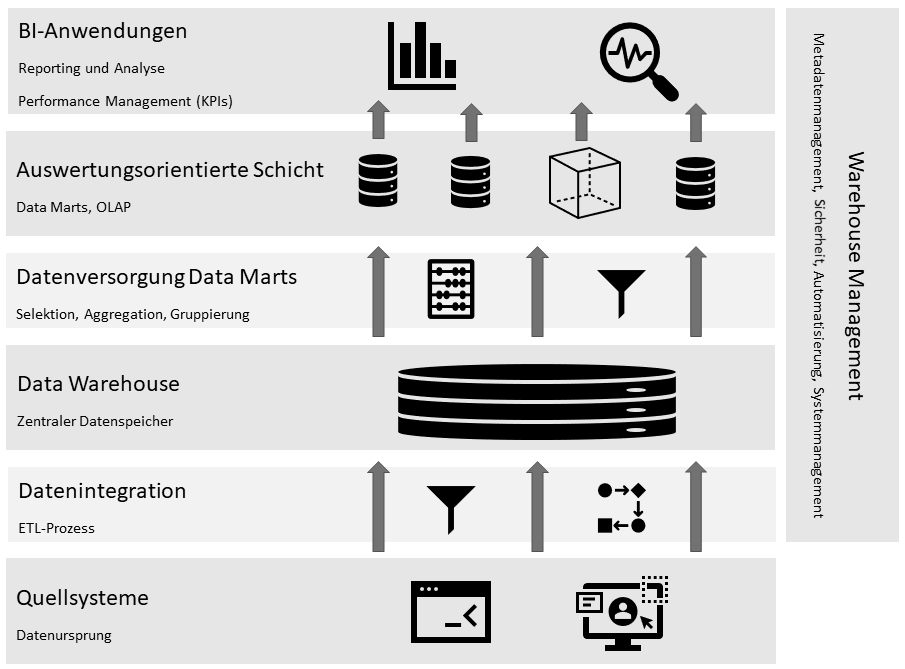
\includegraphics[width=\textwidth]{gfx/aktuelle_onpremise_bi_architektur.png}
 \caption[Aufbau des on-premise BI-Systems]{Aktuelle Architektur des on-premise BI-Systems und Ausgangslage für die Migration in die Cloud \cite{grunwald_business_2009, humm_architektur_2005}}
\label{fig:aktuelle_onpremise_bi_architektur}
\end{figure}

Die einzelnen Schichten werden im Folgenden erläutert \cite{grunwald_business_2009, humm_architektur_2005, kemper_bi-glossar_2008}:
\begin{itemize}
\item \textbf{Quellsysteme} sind der Ursprung aller Daten des BI-Systems. Es kann sich hierbei um interne, sowie externe Quellen handeln. Externe Daten könnten beispielsweise von Marktforschungs- oder Partnerunternehmen stammen. Aktuell werden nur interne Datenquellen abgefragt. Darunter zum Beispiel die Projektmanagement-Software Jira und das Codeanalyse-Tool SonarQube.
\item Die \textbf{Datenintegration} (auch \ac{etl}) ist die Schnittstelle zwischen dem \ac{dwh} und den Quellsystemen. Der \acs{etl}-Prozess beginnt mit dem Extrahieren von operativen Daten aus einem Quellsystem. Darauf folgt eine Transformation, bei der die Daten an syntaktische Anforderungen angepasst werden und semantische Fehler, wenn möglich, behoben werden. Abschließend werden die Daten in das \ac{dwh} zur Speicherung geladen. Für den \acs{etl}-Prozess werden Funktionen vom \textit{Microsoft SQL-Server} und \textit{Powershell-Skripte} genutzt.
\item Das \textbf{Data Warehouse} ist der zentrale Speicherort. Hier werden die Daten strukturiert und langfristig abgelegt. Damit werden sie für weitere Verarbeitungsschritte und Auswertungen zur Verfügung gestellt. In diesem BI-System wird für das Data Warehouse das relationale Datenbankmanagementsystem \textit{Microsoft SQL-Server} verwendet.
\item \textbf{Datenversorgung Data Marts}: Durch den Einsatz von SQL werden in dieser Schicht Daten selektiert, gruppiert und aggregiert. Das Ziel ist die Aufbereitung der Daten für die Data Marts.
\item \textbf{Auswertungsorientierte Schicht}: Data Marts beinhalten spezialisierte Ausschnitte der Daten aus dem \ac{dwh}, in einer für den Zugriff aus den BI-Anwendungen optimierten Form. Ziel ist es, dass für alle Anwendungsfälle eine effiziente Auswertung ermöglicht wird. Verschiedene Data Marts greifen beispielsweise auf die gleichen Daten mit unterschiedlichem Detailgrad und Selektionskriterien zu. Für komplexere Datenanalysen wird das Konzept des \textit{\ac{olap}} angewendet. Dieses soll es Nutzern ermöglichen, auch ohne technische Kenntnisse, Wissen aus dem \ac{dwh} oder den Data Marts zu extrahieren. Das kann durch die Bereitstellung von Ad-hoc-Reports geschehen, welche eine Benutzeroberfläche besitzen, über die mit einfachen Interaktionen flexible Analysen durchgeführt werden können. Dadurch sind keine Kenntnisse in einer Datenbankabfragesprache, wie SQL, notwendig. Die Grundlage für das \ac{olap} sind die sogenannten \ac{olap} Cubes. Unter diesen wird ein multidimensionaler Datenraum verstanden, bei dem die Dimensionen verschiedenen Kontexte, wie zum Beispiel Produkte, Kunden oder Zeit beschreiben. Sowohl die Data Marts als auch die \ac{olap} Cubes sind entweder als View auf das \ac{dwh} oder als eigenständige Datenbanktabelle realisiert.
\item \textbf{BI-Anwendungen} sind die Benutzerschnittstelle zum BI~=System. Hier erfolgen Auswertung und Präsentation. Im aktuellen BI~=System existieren drei Reporting-Anwendungen, die jeweils eine andere Management~=Ebene als Zielgruppe haben. Von den verschiedenen Arten an BI~=Anwendungen werden die Kategorien \textit{Reporting und Analyse} und \textit{Performance Management} abgedeckt. Bei der ersten Kategorie werden standardisierte Berichte in Form von Listen, Tabellen und Grafiken zur Verfügung gestellt. Beim {Performance Management} wird die Unternehmensleistung anhand von ausgewählten \acp{kpi} dargestellt und mit Zielwerten verglichen. Die vorhandenen BI-Anwendungen wurden mit einem internen Reporting~=Framework entwickelt, das auf dem Web~=Framework AngularJS und einer Java"-script Bibliothek zum Erstellen von Visualisierungen basiert.
\item Das \textbf{Warehouse Management} umfasst Aufgaben bezüglich Aufbaus, Pflege und Betrieb des BI-Systems:
\begin{itemize}
\item \textit{Metadatenmanagement}. Verwaltung von Metadaten und Bereitstellung einer gemeinsamen Metadatenbasis für alle Komponenten im System.
\item \textit{Sicherheit}. Authentifizierung und Autorisierung von Benutzern.
\item \textit{Automatisierung}. Event- oder zeitbasierte Ausführung von Prozessen im \ac{dwh}. Zum Beispiel das Ausführen eines ETL-Prozesses zu einer festgelegten Uhrzeit.
\item \textit{Systemmanagement}. Betrieb des \ac{dwh}s gewährleisten. Dazu gehört zum einen die Überwachung von Performance und Auslastung des Systems und zum anderen die Archivierung und Sicherung von Daten.
\end{itemize}
\end{itemize}
\section{Microsoft Azure Cloud} \label{sec:grundlagen:bi_in_der_cloud_mit_azure}
Die Microsoft Azure Cloud wird intern bereits für andere Anwendungsfälle genutzt und ist die einzige Cloud Plattform, die aktuell von der Software AG für die Speicherung und Verarbeitung von Unternehmensdaten zugelassen ist. Mit Microsoft bestehen bereits entsprechende Verträge und die notwendige Zustimmung vom Betriebsrat liegt vor. Die Verwendung eines anderen Cloud~=Providers wäre theoretisch möglich, ist aber in der aktuellen Unternehmensstrategie nicht vorgesehen und würde damit einen deutlich größeren organisatorischen Aufwand bedeuten. Deswegen beschränkt sich diese Arbeit auf Microsoft Azure.

Neben den internen Gründen gibt es aber auch fachliche Argumente für die Wahl von Azure. Hier werden alle Vorteile der Cloud mit gleichzeitig hoher Flexibilität geboten. Die große Auswahl an unterstützten Betriebssystemen, Plattformen und Tools soll es den Kunden ermöglichen, nahezu alle gewünschten Technologien zu verwenden. Des Weiteren hat Microsoft auf der ganzen Welt verteilt Datenzentren und ist auf eine schnelle Disaster Recovery vorbereitet \cite{modi_azure_2020}. Für das hier verfolgt Ziel ist jedoch folgende Aussage aus \citetitle{modi_azure_2020} am wichtigsten "\textit{[...] it provides a host of interconnected services that can pass data among themselves. With such capabilities in place, data can be processed to generate meaningful knowledge and insights}" \cite{modi_azure_2020}. Die Azure Cloud bietet demnach einige Möglichkeiten für die Konstruktion einer BI~=Infrastruktur. Dafür relevante Grundlagen werden im Folgenden beschrieben.

\subsection{Business Intelligence in Azure} \label{subsec:grundlagen:azure:bi}
In der Cloud wird eine Vielzahl an Ressourcen, wie virtualisierte Hardware oder Software, zur Verfügung gestellt. Diese können dynamisch konfiguriert und skaliert werden, sodass immer die benötigte Leistung zur Verfügung steht. Die Azure Cloud ist eine Sammlung an solchen Ressourcen, die sich aktuell in 22 Kategorien einteilen lassen. Manche Dienste können dabei zu mehreren Kategorien gehören. Für den Entwurf der neuen BI~=Architektur werden Dienste aus den folgenden Kategorien in Betracht gezogen \cite{chilberto_building_2020}:
\begin{itemize}
\item \textbf{Integrations}~=Dienste können eingesetzt werden, um Daten aus on~=premise oder Cloud Quellsystemen zu extrahieren.
\item \textbf{Datenbank}~=Dienste sind unter anderem relationale Datenbanken, wie Azure SQL, MySQL und PostgreSQL. Eine Alternative dazu ist die NoSQL~=Datenbank Azure Cosmos DB, welche mehrere Datenmodelle unterstützt.
\item \textbf{Speicher}~=Dienste sind in verschiedenen Formen und Ausprägungen vorhanden und können nach individuellen Anforderungen ausgewählt werden. Das ermöglicht es, eine große Menge an Daten, die sowohl strukturiert als auch unstrukturiert sein können, möglichst günstig abzuspeichern.
\item \textbf{Analyse}~=Dienste helfen, die benötigten Erkenntnisse aus den Daten zu gewinnen.
\item \textbf{KI und Machine Learning} ermöglicht komplexere Analysen. Zum Beispiel können, basierend auf historischen Daten, Vorhersagen über die Zukunft getroffen werden. Diese können beispielsweise genutzt werden, um die zukünftige Entwicklung von \acp{kpi} abzuschätzen.
\item \textbf{Identitäts}~=Dienste werden genutzt, um sicherzustellen, dass nur berechtigte Nutzer Zugriff auf Anwendungen und Daten erhalten.
\item \textbf{Netzwerk}~=Dienste werden verwendet, um eine (sichere) Verbindung zwischen den verschiedenen Ressourcen herzustellen.
\item \textbf{Sicherheit} ist ein wichtiges Kriterium für Cloud~=Systeme. Azure stellt unter anderem Dienste zum Erkennen von Sicherheitsrisiken und zur Überwachung bereit.
\item \textbf{Verwaltung und Governance} umfasst Dienste zur Automatisierung, sowie zur Verwaltung und Überwachung der Cloud~=Ressourcen. Dazu gehört das Erstellen von Backups, sowie das Monitoring von Anwendungen, der Infrastruktur und den dadurch entstehenden Kosten.
\item \textbf{Migrations}~=Dienste sollen beim Umstieg von on~=premise zu Cloud Ressourcen unterstützen. Sie könnten zum Beispiel eingesetzt werden, um Daten aus dem bestehenden \ac{dwh} in eine Cloud Alternative zu übertragen.
\end{itemize}
Beim Vergleich der Azure Kategorien mit den funktionalen Schichten des on~=premise BI~=Systems decken die \textit{Integrations~=Dienste} die Funktionalität der \textit{Datenintegration} ab. Das \ac{dwh} kann in Azure entweder mit den \textit{Datenbank~=}, den \textit{Speicher~=Diensten} oder einer Kombination von beiden ersetzt werden. Die \textit{Analyse~=Dienste} entsprechen der \textit{auswertungsorientierten Schicht} und den \textit{BI~=Anwendungen} des on~=premise Systems. Zusätzlich neue Auswertungsmöglichkeiten bieten die Dienste aus \textit{KI und Machine Learning}. Die Kategorien \textit{Identität}, \textit{Netzwerk}, \textit{Sicherheit} und \textit{Verwaltung und Governance} sind vergleichbar mit dem \textit{Warehouse Management}.

\subsection{Dienste für Sicherheit und Datenschutz} \label{subsec:grundlagen:azure:sicherheitUndDatenschutz}
Neben den Azure Diensten zur Erfüllung der funktionalen Anforderungen, die erst in Abschnitt~\ref{sec:konzeption:evaAuswertung} ausgewählt werden, sollen weitere Dienste für die Sicherheit und den Datenschutz beim Entwurf der neuen BI~=Architektur berücksichtigt werden.

\subsubsection{Azure Policy} \label{subsec:grundlagen:azure:sicherheitUndDatenschutz:ap}
Mit \textit{Azure Policy} kann die Einhaltung bestimmter Compliance Anforderungen für alle Azure Ressourcen erzwungen werden. Dies wird für das System regelmäßig überprüft. Dazu werden zunächst die einzuhaltenden Parameter, wie beispielsweise der Serverstandort, festgelegt. So kann der Versuch eine Ressource zu erstellen, die gegen die festgelegten Compliance Standards verstößt, verhindert werden. Durch \textit{Azure Policy} kann also eine konsistente Einhaltung der Compliance im gesamten BI~=System sichergestellt werden \cite{stefanovic_azure_2021}.

\subsubsection{Azure Key Vault} \label{subsec:grundlagen:azure:sicherheitUndDatenschutz:keyVault}
Der \textit{Azure Key Vault} ist ein sicherer Cloud~=Speicherplatz für Schlüssel, Passwörter und Zertifikate. Dafür verfügt jedes Rechenzentrum über ein Hardware~=Sicherheitsmodul, welches durch den Einsatz von verschiedenen Sensoren sowohl Hacking~=Attacken als auch physische Zugriffsversuchen erkennen kann. In diesem Fall werden alle Passwörter automatisch von der Festplatte gelöscht. Deswegen liegt immer mindestens eine Kopie der Daten in einem anderen Rechenzentrum vor \cite{haunts_key_2019}.

\subsubsection{Azure Active Directory} \label{subsec:grundlagen:azure:sicherheitUndDatenschutz:aad}
\ac{aad} ist ein cloudbasierter Identitäts- und Zugangsverwaltungsdienst. Durch diesen können sich die Nutzer mit Benutzernamen und Passwort authentifizieren. Für eine erhöhte Sicherheit wird außerdem die Verwendung der inzwischen Standard gewordenen \ac{mfa} unterstützt. Das \ac{aad} ermöglicht die Umsetzung von \ac{rbac}. Mit \ac{rbac} können die Zugriffsrechte einer Identität auf die Azure Ressourcen granular festgelegt werden \cite{stefanovic_azure_2021}. Eine Identität kann dabei ein Benutzer, eine Gruppe, ein \textit{service principal} oder eine \textit{managed identity} sein. \textit{Service principals} können in Anwendungen verwendet werden, um diesen Zugriff auf eine Azure Ressourcen zu gewähren. Ähnlich ist die \textit{managed identiy}, bei der das \ac{aad} einer bestimmten Azure Ressource eine Identität zuweist und diese verwaltet. Dadurch kann die Ressource bei Zugriffsversuchen authentifiziert werden, ohne dass Zugangsdaten manuell verwaltet werden müssen \cite{copeland_security_2021}.

%\subsubsection{Microsoft Defender for Cloud} \label{subsec:grundlagen:azure:sicherheitUndDatenschutz:asc}
% Der \textit{Microsoft Defender for Cloud} (ehemals Azure Security Center) soll einen Überblick über die Sicherheit der gesamten Infrastruktur geben. Dazu gibt es unter anderem ein Sicherheitsrating, das als Maßstab für die Bewertung der Systemsicherheit verwendet werden kann  \cite{buchanan_azure_2022}.
\section{Microsoft Azure Cloud} \label{sec:grundlagen:bi_in_der_cloud_mit_azure}

\subsection{Entscheidung für die Microsoft Azure Cloud} \label{subsec:grundlagen:azure:entscheidungFürAzure}
Microsoft Azure wird intern bereits für andere Anwendungsfälle genutzt und ist der einzige Cloud-Provider, der aktuell von der Software AG für die Speicherung und Verarbeitung von Unternehmensdaten zugelassen ist. Mit Microsoft bestehen bereits entsprechende Verträge und die notwendige Zustimmung vom Betriebsrat liegt vor. Die Verwendung eines anderen Cloud-Providers wäre theoretisch möglich, ist aber in der aktuellen Unternehmensstrategie nicht vorgesehen und würde damit einen deutlich größeren organisatorischen Aufwand bedeuten. Deswegen beschränkt sich diese Arbeit auf die Azure Cloud.

Neben den internen Gründen gibt es aber auch fachliche Argumente für die Wahl von Azure. Hier werden alle Vorteile der Cloud mit gleichzeitig hoher Flexibilität geboten. Die große Auswahl an unterstützten Betriebssystemen, Plattformen und Tools soll es den Kunden ermöglichen, nahezu alle gewünschten Technologien zu verwenden. Des Weiteren hat Microsoft auf der ganzen Welt verteilt Datenzentren und ist auf eine schnelle Disaster Recovery vorbereitet \cite{modi_azure_2020}. Für das hier verfolgt Ziel ist jedoch folgende Aussage aus \citetitle{modi_azure_2020} am wichtigsten "\textit{[...] it provides a host of interconnected services that can pass data among themselves. With such capabilities in place, data can be processed to generate meaningful knowledge and insights}" \cite{modi_azure_2020}. Die Azure Cloud bietet demnach einige Möglichkeiten für die Konstruktion einer BI-Infrastruktur.

\subsection{Business Intelligence in der Cloud} \label{subsec:grundlagen:azure:bi}
In der Cloud wird eine Vielzahl an Ressourcen, wie virtualisierte Hardware oder Dienste, zur Verfügung gestellt. Diese können dynamisch konfiguriert und skaliert werden, sodass immer die benötigte Leistung zur Verfügung steht. Microsoft Azure ist eine Sammlung an solchen Ressourcen, die sich aktuell in 22 Kategorien einteilen lassen. Manche Dienste können dabei zu mehreren Kategorien gehören. Für den Entwurf der neuen BI-Architektur werden Dienste aus den folgenden Kategorien in Betracht gezogen \cite{chilberto_building_2020}:
\begin{itemize}
\item \textbf{Integrations}~=Dienste können eingesetzt werden, um die Daten aus Cloud und on-premise Anwendungen zu laden.
\item \textbf{Datenbank}~=Dienste sind unter anderem relationale Datenbanken, wie Azure SQL, MySQL und PostgreSQL. Eine Alternative dazu ist die NoSQL-Datenbank Azure Cosmos DB, welche mehrere Datenmodelle unterstützt.
\item \textbf{Speicher}-Dienste sind in verschiedenen Ausprägungen vorhanden und können nach den individuellen Anforderungen ausgewählt werden. Ziel ist es, eine große Menge an Daten, die sowohl strukturiert als auch unstrukturiert sein kann, möglichst günstig abzuspeichern.
\item \textbf{Analyse}-Dienste helfen, die benötigten Erkenntnisse aus den Daten zu gewinnen.
\item \textbf{KI und Machine Learning} ermöglicht komplexere Analysen. Zum Beispiel können, basierend auf historischen Daten, Vorhersagen über die Zukunft getroffen werden. Diese können beispielsweise genutzt werden, um die zukünftige Entwicklung von KPIs abzuschätzen.
\item \textbf{Identitäts}-Dienste werden genutzt, um sicherzustellen, dass nur berechtigte Nutzer Zugriff auf Anwendungen und Daten erhalten.
\item \textbf{Netzwerk}-Dienste werden verwendet, um eine sichere Verbindung zwischen on-premise und Cloud Infrastruktur herzustellen.
\item \textbf{Sicherheit} ist ein wichtiges Kriterium für Cloud-Systeme. Azure stellt hierfür Dienste zur Überwachung der Datensicherheit und zum Erkennen von Sicherheitsrisiken bereit.
\item \textbf{Verwaltung und Governance} umfasst Dienste zur Automatisierung, sowie zur Verwaltung und Überwachung der Cloud-Ressourcen. Dazu gehört das Erstellen von Backups, sowie das Monitoring von Anwendungen, der Infrastruktur und den dadurch entstehenden Kosten.
\item \textbf{Migrations}-Dienste sollen beim Umstieg von on-premise zu Cloud Ressourcen unterstützen. Sie könnten zum Beispiel eingesetzt werden, um Daten aus dem bestehenden \ac{dwh} in eine Cloud Alternative zu übertragen.
\end{itemize}
Beim Vergleich der Azure Kategorien mit den funktionalen Schichten des on-premise BI-Systems decken die \textit{Integrations-Dienste} die Funktionalität der \textit{Datenintegration} ab. Das \ac{dwh} kann in Azure entweder mit den \textit{Datenbank-}, den \textit{Speicher-Diensten} oder einer Kombination von beiden ersetzt werden. Die \textit{Analyse-Dienste} entsprechen der \textit{auswertungsorientierten Schicht} und den \textit{BI-Anwendungen} des on-premise Systems. Zusätzlich neue Auswertungsmöglichkeiten bieten die Dienste aus \textit{KI und Machine Learning}. Die Kategorien \textit{Identität}, \textit{Netzwerk}, \textit{Sicherheit} und \textit{Verwaltung und Governance} sind vergleichbar mit dem \textit{Warehouse Management}.

\subsection{Dienste für Sicherheit und Datenschutz} \label{subsec:grundlagen:azure:sicherheitUndDatenschutz}
Neben den Azure Diensten zur Erfüllung der funktionalen Anforderungen, die erst in Abschnitt~\ref{sec:konzeption:evaAuswertung} festgelegt werden, sollen weitere Dienste für die Sicherheit und den Datenschutz beim Entwurf der neuen BI-Architektur berücksichtigt werden.

\subsubsection{Azure Policy} \label{subsec:grundlagen:azure:sicherheitUndDatenschutz:ap}
Mit \textit{Azure Policy} kann die Einhaltung bestimmter Compliance Anforderungen für alle Azure Ressourcen erzwungen werden. Dies wird für das System regelmäßig überprüft. Dazu werden zunächst die einzuhaltenden Parameter, wie beispielsweise der Serverstandort, festgelegt. So kann der Versuch eine Ressource zu erstellen, die gegen die festgelegten Compliance Standards verstößt, verhindert werden. Durch \textit{Azure Policy} kann also eine konsistente Einhaltung der Compliance im gesamten BI-System sichergestellt werden \cite{stefanovic_azure_2021}.

\subsubsection{Azure Key Vault} \label{subsec:grundlagen:azure:sicherheitUndDatenschutz:keyVault}
Der \textit{Azure Key Vault} ist ein sicherer Cloud-Speicherplatz für Schlüssel, Passwörter und Zertifikate. Dafür verfügt jedes Rechenzentrum über ein Hardware-Sicherheitsmodul, welches durch den Einsatz von verschiedenen Sensoren sowohl Hacking-Attacken als auch physische Zugriffsversuchen erkennen kann. In diesem Fall werden alle Passwörter automatisch von der Festplatte gelöscht. Deswegen liegt immer mindestens eine Kopie der Daten in einem anderen Rechenzentrum vor \cite{haunts_key_2019}.

\subsubsection{Azure Active Directory} \label{subsec:grundlagen:azure:sicherheitUndDatenschutz:aad}
\ac{aad} ist ein cloudbasierter Identitäts- und Zugangsverwaltungsdienst. Durch diesen können sich die Nutzer mit Benutzernamen und Passwort authentifizieren. Für eine erhöhte Sicherheit wird außerdem die Verwendung der inzwischen Standard gewordenen \ac{mfa} unterstützt.

Das \ac{aad} ermöglicht die Umsetzung von \ac{rbac}. Mit \ac{rbac} können die Zugriffsrechte einer Identität auf die Azure Ressourcen granular festgelegt werden \cite{stefanovic_azure_2021}. Eine Identität kann dabei ein Benutzer, eine Gruppe, ein service principal oder eine managed identity sein. Service principals können Azure Diensten zugewiesen werden, um diesen Zugriff auf andere Ressourcen zu gewähren. Eine managed identiy erfüllt den gleichen Zweck, jedoch müssen damit keine Zugangsdaten verwaltet werden, da dies vom \ac{aad} übernommen wird \cite{copeland_security_2021}.

%\subsubsection{Microsoft Defender for Cloud} \label{subsec:grundlagen:azure:sicherheitUndDatenschutz:asc}
% Der \textit{Microsoft Defender for Cloud} (ehemals Azure Security Center) soll einen Überblick über die Sicherheit der gesamten Infrastruktur geben. Dazu gibt es unter anderem ein Sicherheitsrating, das als Maßstab für die Bewertung der Systemsicherheit verwendet werden kann  \cite{buchanan_azure_2022}.
\section{Spezifikation der Anforderungen}
Die Anforderungen an die neue BI~=Architektur werden in iterativen Meetings mit den Interessensgruppen festgelegt. Eine besondere Herausfor\-der\-ung hierbei ist es, dass die Anforderungsanalyse unvoreingenommen durchgeführt wird. Die Anforderungen sollten weder aus der aktuellen BI~=Lösung noch aus individuellen Lösungsideen abgeleitet werden. Stattdessen sollten sie sich auf die Essenz des Systems beziehen, also den geschäftlichen Grund für den Einsatz des BI~=Systems \cite[vgl.][]{robertson_mastering_2013}.

Als Grundlage für die Anforderungsspezifikation wird eine aktuelle Version des \citetitle{robertson_volere_2020}\textit{s} \cite{robertson_volere_2020} verwendet. Dieses gibt eine grundlegende Struktur und Kategorisierung vor. Hier wird außerdem Wert daraufgelegt, dass beim Beschreiben einer Anforderung ein Testkriterium festgelegt wird. Dadurch werden die Anforderungen messbar und es kann später eindeutig festgestellt werden, ob sie erfüllt wurden. Abgesehen davon werden jedoch nur die Bestandteile der Vorlage übernommen, die für die Evaluation in Abschnitt~\ref{sec:evaluation} als relevant angesehen werden.

Weggelassen wurden Anforderungen an die Benutzerfreundlichkeit und kulturelle Anforderungen, weil für den Endnutzer Reports die einzige Schnittstelle zum BI-System sind. In dieser Arbeit steht jedoch die Architektur im Vordergrund, deswegen ist nur die grundsätzliche Möglichkeit, vielfältige Reports zu erstellen, wichtig. Es ist hier nicht vorgesehen, die Reports zu optimieren. Auch operative und umweltbezogene Anforderungen sind für die Evaluation nicht relevant, da kein Release geplant ist und alle Azure Dienste in einer vergleichbaren physikalischen Umgebung laufen.
\section{Verwandte Arbeiten} \label{ch:verwandteArbeiten}
Bereits 2011 wurden von \citeauthor{ouf_cloud_2011} die Vorteile von Cloud gegenüber on-premise BI beschrieben und eine Architektur vorgeschlagen. Die Beschreibung ist allerdings kurz und abstrakt gehalten. Es wird weder auf das Vorgehen beim Entwurf noch auf eine konkrete Umsetzung eingegangen \cite[vgl.][]{ouf_cloud_2011}. Ein ähnliches Vorgehen wie hier kann in \citetitle{oliver_norkus_rabic_2016} gefunden werden. Die Auswahl der Dienste erfolgt basierend auf Anforderungen und ob diese wirklich erfüllt werden, wird mit einem Prototyp validiert. Im Unterschied zu dieser Arbeit wurde eine Cloud Plattform von \textit{SAP} gewählt und die Beschreibung ist deutlich abstrakter \cite[vgl.][]{oliver_norkus_rabic_2016}. In \citetitle{borosch_cloud_2021} wird die Umsetzung einer Referenzarchitektur aus Azure Diensten detailliert behandelt. Diese unterscheidet sich durch andere Anforderungen und damit den verwendeten Diensten. Außerdem wird beim Entwerfen der Architektur anders vorgegangen, als in dieser Arbeit. Dort wird schrittweise durch das Hinzufügen weiterer Dienste, eine immer komplexere und mächtiger werdende Architektur entworfen. Die Auswahl der verwendeten Dienste wird allerdings nur mit der Funktionalität begründet und es werden keine Alternativen berücksichtigt \cite[vgl.][]{borosch_cloud_2021}.

Nachdem die wichtigsten Begriffe und Grundlagen vorgestellt wurden, wird in den nächsten zwei Kapiteln ein Cloud-BI System entworfen und umgesetzt. Hervorzuheben ist dabei die Auswahl der Azure Dienste, da für die einzelnen Aufgaben nicht immer die naheliegendste Lösung gewählt wird, sondern verschiedene Alternativen betrachtet und in Bezug zu der Anforderungsspezifikation bewertet werden. Eine weitere Besonderheit ist, dass in Kapitel~\ref{ch:praktischeUmsetzung} nicht nur die Umsetzung eines Prototyps beschrieben wird, sondern auch darauf eingegangen wird, wie eine Migration mit möglichst geringen Aufwand durchgeführt werden kann.
%\chapter{Konzeption eines Cloud BI-Systems}
\label{ch:konzeption}
Die in Abschnitt~\ref{sec:grundlagen:bi_in_der_cloud_mit_azure} beschriebenen Kategorien enthalten eine Vielzahl an Diensten und Ressourcen, die potenziell im neuen BI-System eingesetzt werden könnten. Durch eine Evaluation soll hieraus eine geeignete Auswahl getroffen werden. Anschließend wird aus den ausgewählten Komponenten eine vollständige BI-Architektur entworfen.

\section{Anforderungen}
\label{sec:anforderungen}
Im Folgenden soll ein kurzer Überblick über die wichtigsten Anforderungen gegeben werden. Eine vollständige Anforderungsspezifikation kann in Anhang~\ref{ch:anforderungsspezifikation} gefunden werden. 

\subsection{Funktionale Anforderungen}
Es sollen Daten aus verschiedenen on-premise und Cloud Quellsystemen integriert werden können und die extrahierten Daten müssen langfristig gespeichert werden. Auf den gespeicherten Daten sollen automatisierte Analysen und Auswertungen durchgeführt werden können. Die Ergebnisse der Auswertungen sollen visualisiert in Reports angezeigt werden. Neben den fest definierten Auswertungen sollen auch Self-Service-Reports bereitgestellt werden. Außerdem soll die Möglichkeit bestehen, das BI-System um fortgeschrittene Analysen mit Machine Learning zu erweitern, ohne dass grundlegende Veränderungen an der Architektur vorgenommen werden müssen. Die gespeicherten Daten sollen nach festen Regeln automatisch klassifiziert werden, da dies beeinflusst wer Zugriff auf die Daten haben darf. Laut DSGVO Art. 30 ist es erforderlich ein \textit{Verzeichnis von Verarbeitungstätigkeiten} zu führen. Diese Dokumentation aller Übertragungen und Verarbeitungsschritte der Daten soll automatisiert werden. 

\subsection{Nicht-funktionale Anforderungen}
Zu den wichtigsten Anforderungen an Cloud-Systeme gehören die Sicherheit und der Datenschutz \cite{gurjar_cloud_2013}. Daher soll das neue System bestmöglich vor Angriffen geschützt sein. Daneben soll das in DSGVO Art. 17 geforderte \textit{Recht auf Vergessenwerden}, effizient ausgeführt werden können. Eine zuverlässige Authentifizierung und Autorisierung der Nutzer ist ebenfalls unumgänglich. Für alle Daten und Informationen muss sichergestellt werden, dass nur berechtigte Personen diese sehen können. Worauf ein Mitarbeiter Zugriff haben darf, ist abhängig von seiner Rolle im Unternehmen und seinem regionalen Standort. Im Fehlerfall soll ein zuständiges Team benachrichtigt werden und die aufgetretenen Fehler sollen durch eine Protokollierung leicht nachvollziehbar sein. Ein weiteres Kriterium ist die Verwendung von möglichst wenig unterschiedlichen Technologien. Dadurch soll der Wartungsaufwand und die Anzahl der hierfür notwendigen Personen minimiert werden.
\section{Evaluation von Azure Diensten} \label{sec:evaluation}
Im Folgenden sollen einige Azure Dienste, die im Rahmen einer Literaturrecherche ausgewählt wurden, evaluiert werden, mit dem Ziel, aus den gewonnen Erkenntnissen ein BI-System zu entwerfen, dass die festgelegten Anforderungen erfüllt. Dienste, die innerhalb der nächsten fünf Jahre eingestellt werden, wurden vorab ausgeschlossen und Funktionen, die sich noch in der Preview befinden, werden als nicht existent betrachtet. 

Die untersuchten Dienste werden jeweils kurz vorgestellt und es wird auf die wichtigsten Funktionen, Vor- und Nachteile eingegangen, die in bestehender Literatur und den jeweiligen Dokumentationen gefunden werden konnten.

\subsection{Azure Table Storage} \label{sec:grundlagen:azure_dienste:tableStorage}
Der NoSQL-Dienst Table Storage gehört zu den günstigsten Speichermöglichkeiten in Azure. Die Daten werden als Schlüssel/Wert-Paare in Tabellen gespeichert, diese sind jedoch nicht relational und können nicht miteinander gejoint werden. Eine Tabelle besteht aus einer oder mehreren Partitionen und eine Partition besteht aus ein oder mehreren Zeilen. Auf jeden Tabelleneintrag kann über einen eindeutigen Schlüssel zugegriffen werden. Dieser ist eine Kombination aus Partitions- und Zeilen-Schlüssel. Die Partitionierung über mehrere Server ermöglicht es Datenmengen im dreistelligen Terabyte Bereich zu speichern \cite{reagan_web_2018}.

Die gespeicherten Daten werden standardmäßig mit 256-AES verschlüsselt und sind dadurch ohne zusätzlichen Aufwand geschützt \cite{soh_microsoft_2020}. 

Zum Abfragen der Daten gibt es verschiedene Möglichkeiten. Am schnellsten ist die \textit{point query} bei der Partitions- und Zeilen-Schlüssel angegeben werden. Daneben gibt es verschiedene Bereichsabfragen, die entweder die Tabellen einer Partition, mehrerer oder aller Partitionen scannen. Innerhalb der gleichen Partition werden außerdem Transaktionen unterstützt.

Die \textit{Azure Storage Client Library} bietet die Möglichkeit fehlgeschlagene Abfragen, zum Beispiel wegen eines Server-Timeouts, automatisch zu wiederholen. Alternativ kann beim Zugriff über REST API eine eigene Wiederholungslogik bei Fehlern implementiert werden.

Die größte Schwäche von Table Storage ist, dass nur auf den Partitions- und Zeilen-Schlüssel ein Index angelegt wird. Performante Abfragen auf andere Attribute als die Schlüssel sind daher nicht möglich \cite{reagan_web_2018}.

\textbf{Fazit}: Table Storage ist günstig, schnell und kann problemlos die Anforderungen an die zu speichernde Datenmenge erfüllen. Jedoch werden für die Auswertungen im aktuellen System sowohl Tabellen-Joins als auch Abfragen von Attributen, die nicht der indexierte Schlüssel sind, verwendet. Eine daraus folgende Einschränkung ist, dass das \textit{Recht auf Vergessenwerden} nur umgesetzt werden kann, wenn eine eindeutige Kunden- bzw. Personenkennzeichnung als Schlüssel verwendet wird.

Daher ist der Table Storage hier nicht geeignet, um als alleinstehende Speicherlösung genutzt zu werden. Er könnte jedoch als Ergänzung zum Kosten sparen eingesetzt werden \cite[vgl.][]{reagan_web_2018}. 

\subsection{Azure SQL} \label{sec:grundlagen:azure_dienste:sql}
Azure SQL ist eine Produktfamilie von relationalen Datenbanken, die basierend auf Abstraktion und Zugriff in Betriebssystem-, Server- und Datenbankebene eingeteilt werden kann:

\begin{itemize}
\item \textbf{SQL Server auf Azure-VMs} stellt einen Microsoft SQL Server auf Betriebssystemebene bereit. Es handelt sich um eine virtuelle Maschine, auf der ein SQL Server installiert ist. Dadurch hat der Nutzer auf der einen Seite mehr Kontrolle, auf der anderen aber auch mehr Verantwortung und Konfigurationsaufwand. 
\item Wird nur die Kontrolle über den SQL-Server, aber nicht über das Betriebssystem benötigt, eignet sich die \textbf{Verwaltete Azure SQL-Instanz}. Diese bietet nahezu alle Features einer normalen SQL-Server-Instanz. Eines dieser Features ist zum Beispiel Machine Learning mit R oder Python auf die Daten anzuwenden \cite{ericson_was_2021}.
\item Die \textbf{Azure SQL-Datenbank} ist eine relationale Datenbank in der Cloud die ohne Verwaltungsaufwand genutzt werden kann. Es handelt sich damit um die höchste Abstraktionsebene, die dann eingesetzt werden kann, wenn weder Kontrolle über die Instanz noch Features auf Serverebene benötigt werden.
\end{itemize}
\cite{mauri_azure_2021}

Die Abfragesprache T-SQL bietet einige Möglichkeiten zum Transformieren und Auswerten der Daten, wie zum Beispiel die Umwandlung in einen anderen Datentyp oder die Durchführung von mathematischen Berechnungen. Für den Umgang mit möglicherweise auftretenden Fehlern kann in T-SQL eine Try/Catch-Logik genutzt werden \cite[vgl.][]{kellenberger_beginning_2021}.

Ruhende Daten werden von Azure SQL-Datenbank automatisch verschlüsselt. Die Konsistenz der gespeicherten Daten kann durch die Wahl eines geeigneten Datenmodells erreicht werden \cite{reagan_web_2018}. Auch die Autorisierung über das \ac{aad} mit \ac{rbac} wird von Azure SQL unterstützt \cite{wolter_authorize_2021}.

Es gibt zwei Möglichkeiten, die Performance bei Bedarf zu verbessern. Solange die oberste Preisstufe noch nicht erreicht wurde, ist das Erhöhen dieser der einfachste Weg, Leistung und Speicherkapazität zu steigern. Azure führt dazu alle notwendigen Schritte zum Ändern der Datenbank automatisch im Hintergrund aus. Eine automatische Skalierung nach Bedarf wird jedoch nicht unterstützt. Die zweite deutlich komplexere Option ist die horizontale Partitionierung der Daten auf mehrere SQL-Instanzen (Sharding) \cite{reagan_web_2018}.

\textbf{Fazit}: Der größte Vorteil von Azure SQL ist, dass alle zu migrierenden Daten bereits in einem relationalen Datenmodell vorliegen. Zusätzlich eignet sich die T-SQL für einfache Datenverarbeitungen, wobei auch hier die meisten Skripte aus dem Bestandssystem übernommen werden könnten.

Von den drei Azure SQL Diensten werden nur die verwaltete SQL-Instanz und die SQL-Datenbank für das neue BI-System in Erwägung gezogen, da die Kontrolle auf Betriebssystemebene nicht benötigt wird. Welcher dieser beiden Dienste besser geeignet ist, hängt besonders davon ab, wie die zusätzlichen Funktionen der verwalteten SQL-Instanz gegenüber der SQL-Datenbank in Verbindung mit zusätzlichen Diensten zu werten sind. 

\subsection{Azure Cosmos DB} \label{sec:grundlagen:azure_dienste:cosmosDB}
Bei diesem Dienst handelt es sich um eine NoSQL-Datenbank, die mehrere Datenmodelle, wie Schlüssel-Wert, Dokument oder Graph, unterstützt. Intern werden die Daten als Dokumente im JSON-Format gespeichert. Solange die Daten sich in Ruhe befinden, sind sie verschlüsselt.

Dabei werden verschiedene APIs zum Zugriff auf die Daten angeboten, wie unter anderem DocumentDB SQL (bietet gängige SQL-Abfragefunktionen), MongoDB, Apache Casandra, Graph und Table (bietet gleiche Funktionalität wie Azure Table). Auch das Konsistenzniveau der Daten kann aus fünf Ebenen, von starker bis eventueller Konsistenz, gewählt werden.

Das Feature \textit{Turnkey Global Distribution} beschreibt die automatisierbare Replikation über verschiedene Regionen. Dadurch können weltweit geringe Latenzzeiten gewährleistet werden. Die einzige notwendige Konfiguration ist dabei die Auswahl der gewünschten Regionen, alles andere wird automatisch von Azure übernommen.

Sowohl der Durchsatz, der in \acp{ru} gemessen wird, als auch die Speicherkapazität kann dynamisch nach Bedarf skaliert werden. Davon sind auch die entstehenden Kosten abhängig.
\cite{guay_paz_microsoft_2018}\cite{mrzyglod_hands-azure_2018}

Der Zugriff auf Cosmos DB kann über \ac{aad} und \ac{rbac} kontrolliert werden \cite{weiss_azure_2021}.

\textbf{Fazit}: Besonders das gleichzeitige Verwenden mehrerer Datenmodelle macht aus Cosmos DB eine interessante Möglichkeit für ein BI-System. Für alle gespeicherten Daten, kann das Modell verwendet werden, dass für den benötigten Anwendungsfall optimal ist. Von der gewählten API sind auch die Möglichkeiten zur Datenfernverarbeitung mit diesem Dienst abhängig. Während die Table API dafür ungeeignet ist, sind mit der SQL-Artigen DocumentDB Transformationen und Auswertungen möglich.

\subsection{Azure Data Lake Gen 2} \label{sec:grundlagen:azure_dienste:dataLake}
\acp{blob} sind unstrukturierte Dateien, die sich nicht zum Speichern in einer Datenbank eignen. Eine kostengünstige Möglichkeit, diese in der Cloud abzulegen, ist der Blob Storage. Auf diesen Dienst baut auch der Data Lake Gen 2 auf, welcher für die Analyse der gespeicherten Daten spezialisiert wurde. Organisieren lassen sich die Dateien in einer hierarchischen Ordnerstruktur \cite{soh_microsoft_2020}.

Der Data Lake ist in verschiedene Schichten eingeteilt. Die oberste Ebene bezieht sich auf die Umgebung, wie zum Beispiel Entwicklung, Test oder Produktion. Innerhalb einer Umgebung kann es einen oder mehrere Storage Accounts geben. In dieser Schicht können Einstellungen, wie die Leistungsstufe, oder die Replikationsmethode gesetzt werden. Die Leistungsstufe bestimmt unter anderem, ob ein günstiger Magnetspeicher oder Solid-State-Festplatten für schneller Lese-/Schreib-Prozesse, verwendet wird. Die nächste Schicht ist das Dateisystem in dem sich die Verzeichnisse und Dateien befinden.

Azure Data Lake Gen 2 verschlüsselt die Daten, während sie sich in Ruhe befinden oder bewegt werden, automatisch. Der Zugriff auf den Data Lake kann auf der Storage Account Ebene über \ac{rbac} gesteuert werden. Für eine granulare Zugriffskontrolle können auf der Verzeichnis/Ordner-Ebene POSIX-Artige Zugriffssteuerungslisten (ACLs) konfiguriert werden.

Mit Hilfe der Dienste \ac{adf} oder Azure Databricks kann der Data Lake um das Open-Source-Layer \textit{Delta Lake} erweitert werden. Durch dieses wird aus dem Data Lake eine ACID-konforme Speicherlösung und die Atomarität, Konsistenz, Isolation und Dauerhaftigkeit der Daten kann garantiert werden \cite{lesteve_definitive_2021}. Der Delta Lake ermöglicht es außerdem deutlich effizienter Personendaten bei Bedarf zu löschen \cite{brown_best_2021}.

\textbf{Fazit}: Die Verwendung von Azure Data Lake Gen 2 ist sinnvoll, wenn viele oder große \ac{blob}-Dateien gespeichert werden müssen. Dies ist zunächst kein Anwendungsfall, der im neuen BI-System benötigt wird. Sollten sich die Anforderungen in Zukunft ändern, könnte Data Lake jedoch eine gute Ergänzung zu einer Datenbank sein.

\subsection{Azure Logic Apps} \label{sec:grundlagen:azure_dienste:logicApps}
Mit diesem Dienst können automatisierte Workflows zur Datenintegration erstellt werden. Die Workflows sind sehr anpassungsfähig und es steht eine Vielzahl an vorgefertigten Konnektoren zur Verfügung \cite{kumar_serverless_2019}.

Ein Logic Apps Workflow besteht aus zusammenhängenden Aktivitäten, in einer bestimmten Reihenfolge. Die erste Aktivität ist immer ein Trigger, der die Ausführung des Workflows startet. Alle weiteren Aktivitäten sind Aktionen, die jeweils eine einzige Aufgabe erfüllen und nacheinander abgearbeitet werden. Hier können auch die Konnektoren verwendet werden, mit denen eine Verbindung zu externen Ressourcen aufgebaut werden kann. Die Verbindung ist zu Cloud und on-premise Ressourcen möglich. Die Workflows können über eine Drag-and-Drop-Benutzeroberfläche erstellt werden \cite{modi_azure_2020}.

Auch Datentransformationen, wie mathematische Berechnungen und Textmanipulationen, sind in einem Workflow mit möglich. Dazu werden \ac{dax} Funktionen verwendet, welche mit Excel Formeln vergleichbar sind \cite{bennett_enterprise_2021}.

Beim Eintreten von Fehlern werden vorher festgelegte Wiederholungsrichtlinien ausgeführt. Es ist ebenfalls möglich, nach einem aufgetretenen Fehler, mit einer alternativen Aktion fortzufahren, um zum Beispiel eine zuständige Person per E-Mail zu informieren \cite{fan_handle_2021}.

Für eine ausreichende Sicherheit werden die Daten während der Übertragung mit TLS und im Ruhezustand verschlüsselt. Auch die Authentifizierung mit \ac{aad} und Autorisierung durch \ac{rbac} wird unterstützt \cite{baldwin_azure_2021-1}. 

\textbf{Fazit}: Mit den angebotenen Konnektoren von Logic Apps, können alle hier benötigten Quellsysteme integriert werden \cite[vgl.][]{fan_verwaltete_2021}. Vor dem Speichern können die Daten bei Bedarf verarbeitet werden. Dieser Dienst ist außerdem performant und benötigt für die meisten Ausführungen nur wenige Sekunden \cite{bennett_enterprise_2021}. Durch die Manipulationsmöglichkeiten wäre auch ein Verarbeitungsschritt möglich, in dem nach festen Regeln Attribute zur Datenklassifikation ergänzt werden.

\subsection{Azure Data Factory} \label{sec:grundlagen:azure_dienste:dataFactory}
\ac{adf} ist ein Datenintegrationsdienst, der für on-premise und Cloud Systeme genutzt werden kann. Der Dienst wurde speziell für den gemeinsamen Einsatz mit anderen Diensten entwickelt und übernimmt dabei die Bewegung, Transformation und Verarbeitung der Daten, zwischen den unterschiedlichen Systemen \cite{klein_iot_2017}.

Der ETL-Prozess wird als Pipeline implementiert. Eine Pipeline ist eine Sammlung von Aktivitäten zum Bewegen und Transformieren von Daten. 

Die \textit{Azure Data Factory User Experience} bietet eine webbasierte IDE für die visuelle Erstellung, Planung und Überwachung von Pipelines. Das \textit{Copy Data tool} führt einen schrittweise durch die Erstellung einer neuen Pipeline, die Daten von einer Ressource zu einer anderen verschiebt. Dabei werden unter anderen Datenspeicher- und Computedienste mit der \ac{adf} verknüpft. Die Trennung dieser hat den Vorteil, dass beides unabhängig voneinander nach Bedarf skaliert werden kann.

\ac{adf} besitzt keinen eigenen Speicher, sondern verwendet ausschließlich die verknüpften Dienste. Ein verknüpfter Dienst besteht aus den notwendigen Metadaten für eine Verbindung, beispielsweise die Verbindungszeichenfolge für eine Datenbank. Metadaten, die konkrete Objekte im verknüpften Speicherdienst beschreiben, werden als Dataset definiert. 

Für die Verarbeitung der Daten können verknüpfte Dienste, wie Azure Databricks oder HDInsight verwendet werden. Alternativ bietet eine \textit{integration runtime} Zugang zu internen Rechenressourcen innerhalb von \ac{adf} \cite{swinbank_your_2021}.

\textbf{Fazit}: \ac{adf} könnte im neuen BI-System für die Datenintegration genutzt werden. Im Gegensatz zu Logic Apps setzt dieser Dienst auf die Zusammenarbeit mit weiteren Azure Ressourcen, um den ETL-Prozess durchzuführen, was zu einem komplexeren Gesamtsystem führen könnte.

\subsection{Azure HDInsight} \label{sec:grundlagen:azure_dienste:hdInsight}
Azure HDInsight realisiert Apache Hadoop, als vollständig verwalteten Cloud Dienst. Dazu wird von dem Dienst ein Cluster von virtuellen Maschinen, die das \textit{Hadoop Distributed File System} benutzen, verwaltet. Dieses verteilte Dateisystem ist auf Fehlertoleranz und einen hohen Durchsatz ausgelegt ist.

Hadoop ist eine Sammlung von Open~=Source Komponenten, die für die verteilte Verarbeitung und Analyse großer Datensätze konzipiert wurden. Zum Abfragen, Transformieren und Analysieren von Daten stehen unter anderem folgende Funktionen zur Verfügung:
\begin{itemize}
\item \textit{Hive}: Stellt die SQL-artige Abfragesprache HiveQL zur Verfügung und verwendet ein dynamisches Schema, das erst beim Lesen der Daten angewendet wird. Damit kann HDInsight auch ETL-Prozesse durchführen.
\item \textit{Storm}: Echtzeitverarbeitung von großen Datenströmen 
\item \textit{Pig}: Die prozedurale Sprache Pig Latin ermöglicht es Schemata zu erstellen und Abfragen über Skripte durchzuführen.
\item \textit{MapReduce}: Framework zur parallelen Verarbeitung von Daten auf mehreren Rechnern.
\end{itemize}

Hadoop kann eine hohe Verfügbarkeit bieten und kann je nach Bedarf skalieren, wie viele Rechner verwendet werden. Aufgetretene Fehler können selbständig erkannt werden und wenn notwendig wird die fehlgeschlagene Aufgabe an einen anderen Rechner weitergeben \cite{klein_iot_2017}.

\textbf{Fazit}: Dieser Dienst ist vergleichsweise komplex, da individuelle Konfigurationen notwendig sind. Ein möglicher Anwendungsfall wäre ein ETL-Prozess zwischen einem unstrukturierten Speicher, wie dem Data Lake und einer relationalen Datenbank. \cite[vgl.][]{klein_iot_2017}.

\subsection{Azure Databricks} \label{sec:grundlagen:azure_dienste:databricks}
Azure Databricks setzt Apache Spark als Cloud-Dienst um. Spark ist ein Open-Source Framework für die Big Data Analyse. Im Gegensatz zu Hadoop werden die Daten zur schnelleren Verarbeitung im Arbeitsspeicher vorgehalten \cite{soh_data_2020}.

\subsection{Azure Machine Learning} \label{sec:grundlagen:azure_dienste:machineLearning}
\ac{aml} ist eine Sammlung von Funktionen und Tools zum Arbeiten mit ML-Modellen in einer skalierbaren Cloud-Umgebung. Dafür kann Python, R oder die zero/low code Option \textit{Azure ML designer} verwendet werden.

Von den hier betrachteten Speichermöglichkeiten können entweder Azure SQL-Datenbank oder Data Lake Gen 2 an \ac{aml} angebunden werden \cite{soh_data_2020}.

\textbf{Fazit}: \textit{...}

\subsection{Azure Analysis Services} \label{sec:grundlagen:azure_dienste:analysisServices}
\ac{aas} ist eine Cloud Implementierung des Tools \textit{Microsoft SQL Server Analysis Services}. Der Dienst kann als Semantik-Schicht zwischen \ac{dwh} und Endnutzer agieren. In dieser Funktion können beispielsweise Spalten umbenannt oder irrelevante Werte ausgeblendet werden, damit übersichtliche Reports entstehen. Der Dienst kann jedoch nur mit tabellarischen Datenmodellen umgehen, nicht mit multidimensionalen.

Obwohl ein Data Warehouse die gleichen analytischen Möglichkeiten bietet, kann es sinnvoll sein, Speicher- und Analyseschicht für mehr Flexibilität und weniger Komplexität voneinander zu trennen.

\ac{aas} ermöglicht außerdem die Implementierung von granularen Zugriffsrichtlinie auf Zeilenniveau mit \ac{rbac} in Verbindung mit dem \ac{aad}.

Für effiziente Analysen wird das \textit{Vertipaq Engine} genutzt, welches alle Daten im Arbeitsspeicher ablegt. Um den benötigten Speicher zu reduzieren, werden außerdem verschiedene Algorithmen zum Komprimieren der Daten verwendet.

Ein Analysis Services Modell enthält die Daten und weitere Objekte, wie die daraus berechneten \acp{kpi} \cite{how_beyond_2020}.

\textbf{Fazit}: \ac{aas} könnte als Semantik-Schicht zwischen Daten und Reports genutzt werden. Ob der Dienst einen Mehrwert für die Cloud-BI bieten könnte, hängt besonders von der gewählten Speicherlösung und den damit zur Verfügung stehenden Funktionen zur Datenverarbeitung ab.

\subsection{Power BI} \label{sec:grundlagen:azure_dienste:powerBI}
Power BI ist Microsofts Dienst zum Visualisieren von Daten. Gleichzeitig können \ac{etl}-Prozesse und Auswertungen durchgeführt werden, die auf der gleichen Power Query Engine, wie bei \ac{aas} basieren. Mit Power BI können vorgefertigte und Self-Service Reports erstellt werden.

Power BI besteht aus mehreren Kernkomponenten wie die Entwicklungsumgebung für Reports \textit{Power BI desktop}, oder das webbasierte Portal \textit{Power BI servcice}, wo die veröffentlichten Reports betrachtet werden können.

Zum Erstellen eines Reports wird zunächst eine Datenquelle verknüpft. Hier werden einige Konnektoren angeboten, mit denen unter anderem mit allen hier vorgestellten Speicherlösungen eine Verbindung aufgebaut werden kann. Anschließend kann das dazugehörige Datenmodell in bearbeitet werden. Relationen werden automatisch von Power BI erkannt, es können jedoch manuell weitere hinzugefügt werden. Mit einem vollständigen Datenmodell können anschließend Reports mit Visualisierungen, wie Balkendiagramme, in einer grafischen Benutzeroberfläche erstellt werden. Abschließend wird der Report veröffentlicht und wird in Power BI service angezeigt.

Power BI kann auch eine Liveverbindung zu \ac{aas} aufbauen und Abfragen an diesen Dienst weitergeben, wodurch auf einen vorherigen Import der Daten verzichtet werden kann.
\cite{how_beyond_2020}.

\textbf{Fazit}: Mit Power BI können alle hier benötigten Reporting-Funktionalitäten umgesetzte werden, damit ist es eine geeignete Option für das neue BI-System, um als Schnittstelle zu dem Endnutzer zu fungieren.

\subsection{Azure Synapse Analytics} \label{sec:grundlagen:azure_dienste:synapseAnalytics}
Azure Synapse Analytics (ehemals Azure SQL Data Warehouse) vereint Datenintegration, Data Warehouse und Big Data Funktionalität in einem Dienst. Der Dienst enthält eine SQL-Engine und unterstützt weitere Speicherdienste wie den Azure Data Lake. Dadurch können Daten jeglicher Struktur gespeichert und verarbeitet werden. Durch eine unbeschränkte Skalierbarkeit ist dies für mehrere Petabyte möglich.

Die Weboberfläche \textit{Synapse Studio} ist eine einheitliche Verwaltungsschnittstelle, damit Daten über aufgenommen, untersucht, aufbereitet und für BI- und Machine Learining Anwendungen bereitgestellt werden können. Hier sind beispielsweise SQL-Abfragen möglich, die direkte Verwendung von \nameref{sec:grundlagen:azure_dienste:machineLearning}, oder auch die Erstellung von PowerBI Visualisierungen und Reports.

Für die Datenintegration wird die auf \ac{adf} basierende \textit{Synapse Pipeline} angeboten. Dadurch ist eine einfache Verbindung zu einer Vielzahl von Quellsystemen möglich.

Durch Synapse Spark, welches auf Grundlage von Apache Spark entwickelt wurde, wird die Analyse von großen Datenmengen ermöglicht. Hierfür kann Python, Scala, C\# oder Spark SQL verwendet werden.

Azure Synapse Analytics bietet einige Sicherheitsfunktionen, darunter die automatische Erkennung von Bedrohungen und eine immer aktive Verschlüsselung. Der Zugriff kann auf Spalten- oder Zeilenlevel geregelt werden.
\cite{shiyal_beginning_2021}

\textbf{Fazit}: Azure Synapse Analytics vereint mehrere Technologien und andere Azure Dienste in einem, wodurch die meisten funktionalen Anforderungen an das Cloud-BI-System erfüllt werden könnten. Jedoch ist dieser Dienst vergleichsweise komplex. Es werden einige Funktionalitäten geboten, die besonders für Big Data Anwendungsfälle attraktiv sind, jedoch hier nicht benötigt werden.

\subsection{Azure Purview} \label{sec:grundlagen:azure_dienste:purview}
Purview dient der zentralen Verwaltung der Datengovernance, für Cloud und on-premise Umgebungen. Dabei soll die Datenherkunft leicht nachvollziehbar werden. Die Metadaten zu den Quellen können um Tags und Beschreibungen erweitert werden. Der Dienst kann über die Benutzeroberfläche Purview Studio verwaltet werden. Der Zugriff auf dieses und die Informationen wird über Rollen und das \ac{aad} kontrolliert.

Im Purview Studio können Benutzer neue Datenquellen registriert werden, damit zusätzliche Metadaten zu diesen verwaltet werden können. Durch das Erstellen einer \textit{Scan Rule} können die Datenquellen gescannt werden, wobei die Daten nach vorher definierten Regeln klassifiziert werden. Der Scan kann einmalig oder wiederholt nach Zeitplan ausgeführt werden \cite{lesteve_definitive_2021}. Dadurch wird die Nachvollziehbarkeit der Datenherkunft ermöglicht. Diese umfasst den Ursprung, aber auch alle Verarbeitungen und Bewegungen der Daten \cite{riscutia_data_2021}.

Auch die Übertragung und Speicherung der Daten geschieht in Purview verschlüsselt \cite{baldwin_azure_2021}. 

\textbf{Fazit}: Purview bietet einige Funktionen, die helfen, die Sicherheit und den Datenschutz der BI-Lösung zu verbessern. Purview kann verwendet werden, um die Daten in regelmäßigen Scans zu klassifizieren und dabei den vollständigen Datenfluss zu dokumentieren. Durch die Erweiterung der Metadaten um bestimmte Tags kann Purview zusätzlich dabei helfen, auf Anfrage alle Daten eines Kunden zu löschen.
\section{Entwurf der neuen BI-Architektur}
\label{sec:entwurfBIArchitektur}
Basierend auf dem Ergebnis des vorherigen Abschnitts, wird ein Entwurf für eine vollständige BI-Architektur, in der Azure Cloud, vorgestellt. Dabei wird auf die Verbindung der einzelnen Komponenten, zu einem funktionierenden Gesamtsystem, eingegangen. Insbesondere auch auf die Kommunikation zwischen den einzelnen Komponenten und wie hierbei die Einhaltung von Sicherheit und Datenschutz gewährleistet wird.
%*************************************************************************
% Recommendations
%*************************************************************************
%\part{Empfehlungen zur Erstellung wissenschaftlicher Abschlussarbeiten}
%\label{pt:recommendations}
%*************************************************************************
% Backmatter
%*************************************************************************
% \appendix
%\renewcommand{\thechapter}{\alph{chapter}}
%\cleardoublepage
%\part{Appendix}
%\chapter{Anforderungsspezifikation}\label{ch:anforderungsspezifikation}

%\include{chapters/examples/appendix02}
%*************************************************************************
% Other Stuff in the Back
%*************************************************************************
\cleardoublepage\include{frontbackmatter/Bibliography}
%*************************************************************************
% Game Over: Restore, Restart, or Quit?
%*************************************************************************
\end{document}
%*************************************************************************
